 \documentclass[encoding=utf8,british]{tumphthesis}
% \documentclass[pstricks,siunitx,addfonts,theorem,font=palatino,british]{tumphthesis}
% für Dissertation:
% \documentclass[encoding=utf8,british,dissertation,font=helvet]{tumphthesis}

% Das folgende Paket dient lediglich dazu, den Blindtext "Lorem ipsum ..."
% auszugeben und kann in einer echten Abschlussarbeit natürlich weggelassen 
% (oder auskommentiert) werden.
\usepackage{lipsum}

% Die Metadaten der Abschlussarbeit (Bachelor oder Master) werden auf dem 
% Deckblatt gedruckt und in dem PDF eingetragen.
\subject{Quantum Science and Technology Master's thesis}
\title{Quantum tensor networks for sampling}
%\subtitle{\foreignlanguage{british}{Title in English}}
\author{Simon Botond}
\date{\today}
%\cooperators{Max-Planck-Institut für Physik}

% Alternativ Dissertation:
%\title{Titel der Dissertation}
%\subtitle{\foreignlanguage{british}{Title in English}}
%\author{Sheldon Cooper}
%\date{31.~Juli 2011}
%\DepartmentOrIRC{Fakultät für Physik}
%\DrDegree{der Naturwissenschaften}
%\Vorsitz{Prof. Dr. Patricia Kabelschacht}
%\ErstPrueferin{Prof. Dr. Erwin Brezensaltzer}
%\ZweitPrueferin{PD Dr. habil. Heidelinde Musterfrau}
%\DrittPrueferin{Prof. Dr. }

% Auf der Rückseite des Deckblatts können Themensteller, Zweitgutachter 
% und Tag der mündlichen Prüfung vermerkt werden.
\lowertitleback{Erstgutachter (Themensteller): Dr. Jeanette Miriam-Lorentz\\
Zweitgutachter: Alex Goessmann}

% Die Bibliographie wirde über BibLaTeX mit Biber-Backend erstellt. 
% Sofern vorhanden, wird eine bib-Datei \jobname.bib (i.d.R. also der 
% gleiche Name wie die Hauptdatei nur bib-Endung) automatisch eingebunden.
% Heißt sie anders oder müssen weitere Quelldateien eingebunden werden, so 
% dient dazu der folgende Befehl (auch z.B. bei Verwendung von ShareLaTeX 
% erforderlich, da hier \jobname auf output gesetzt wird)
% \addbibresource{thesis.bib}

\begin{document}
% Ist die Arbeit auf Englisch verfasst, hier die Sprache umschalten. 
% Die Sprache muss als Klassenoption angegeben sein.
\selectlanguage{british}

\frontmatter
\maketitle

%\newpage

\mainmatter

\chapter*{Abstract}

Efficient sampling from complex probability distributions is a cornerstone of modern Artificial Intelligence workflows, enabling 
critical tasks such as probabilistic inference, generative modeling, and optimization. Classical sampling methods, 
including brute force or Markov Chain Monte Carlo methods, face prohibitive computational challenges as the 
dimensionality and logical complexity of target distributions grow. This thesis investigates the potential of 
quantum computing - specifically amplitude amplification algorithms - to overcome these limitations and deliver practical 
advantages for machine learning sampling tasks. Through a systematic methodology, logical connectives and graphical 
models are mapped to quantum circuits via the Tensor network decomposition of their exponential family distributions.
Simulations on up to $\approx 25$ qubits (variables and ancillas together) demonstrate the scalability of quantum amplitude amplification, while 
comparative analyses with classical baselines quantify speedup and a possible turnover point. The results reveal that 
quantum-assisted sampling achieves quadratic speedups for structured distributions, though hardware constraints and 
noise pose significant challenges. This work bridges quantum computing and machine learning by formalizing a 
framework for integrating quantum sampling into classical workflows, offering a pathway toward scalable probabilistic 
inference in AI systems.

\tableofcontents

\chapter{Introduction}
    \section*{Motivation and Background}
    \label{sect:Intro_mot_back}
        Sampling is an essential part of a machine learning algorithm. Whenever the program makes a 
        decision, handles predictions with uncertainty or gives solutions to a problem, it is a form of sampling 
        from a vast set of information. This set is usually called data or knowledge.
        Sampling therefore is fundamental in enabling probabilistic inference, uncertainty quantification, 
        and optimization in high-dimensional spaces. As models are increasingly sophisticated - incorporating rich logical structures 
        or large graphical dependencies - their complexity escalates and the computational demands of sampling algorithms 
        grow exponentially. Classical methods, while foundational, struggle to balance accuracy and efficiency in 
        high-dimensional or multimodal distributions. Quantum computing, with its inherent parallelism and interference 
        capabilities suggest that quantum algorithms could offer speedups for certain sampling 
        tasks. This motivates a systematic investigation of their applicability and impact for artificial intelligence~\cite{Mansky_2023}\cite{PubMed}. 
        This thesis explores the intersection of quantum computing and AI, focusing on how quantum 
        amplitude amplification can revolutionize sampling tasks in artificial intelligence.
    The following sections elaborate on the background and motivation, objectives, challenges, and the structure 
    of this work.
    
    \section*{Machine Learning and Artificial Intelligence}
    \label{sect:Intro_ML_AI}
        Machine Learning (ML) and Artificial Intelligence (AI) are transformative fields that enable systems to learn patterns, 
        make predictions, and automate decision-making using data and knowledge~\cite{AI_modern}. 
        
        Machine Learning focuses on developing algorithms that build models from training data to optimize tasks such as classification, 
        regression, and optimization. 

        Artificial Intelligence, on the other hand, is a broader field that generalizes these capabilities to encompass not only learning but also reasoning, 
        planning, and knowledge representation. It involves sophisticated approaches to mimic human cognitive functions such as symbolic logic or heuristic search. 

        Together, they are revolutionizing various industries, from healthcare and finance to autonomous vehicles and personalized digital assistants, 
        by enabling smarter, more efficient, and adaptive technologies.
        
        In the financial domain, ML models analyze massive datasets. These can include market prices, transaction histories or risk indicators, to detect anomalies, 
        forecast trends, and manage portfolios. AI augments these tasks with strategic reasoning and adaptive autonomy, driving advances in 
        for example fraud detection or investment optimization. The uncertainty in financial and other real-world territories 
        necessitates robust modeling of data distributions, a challenge met by probabilistic methods and advanced sampling techniques~\cite{FinanceMLAI}.

    \section*{Data Representation in ML and AI}
    \label{sect:Intro_Data_Rep}
        Data constitutes the foundational resource for ML and AI systems. It may exist as numerical records, time series, images, text documents, 
        or relational graphs. The efficiency of learning and inference depend on how this data is represented. Common approaches include tabular datasets, feature vectors, 
        relational graphs, and tensor networks, each suited for capturing structure, dependencies, and semantics within data.

        Knowledge builds upon data by explicitly encoding recognized patterns, relationships, and rules. These are either uncovered through analysis or are previously contributed. 
        This higher-level representation often takes the form of logical formulas, graphical models (such as Bayesian networks), or advanced tensor structures. Effectively, 
        knowledge can be seen as data made explicit: enriched with well-defined dependencies, constraints, and connections. The representation chosen determines both the 
        performance and expressiveness of ML/AI algorithms, especially when combining reasoning, prediction, and uncertainty quantification.

    \section*{Sampling: Concepts and Role in ML/AI}
    \label{sect:Intro_Sampling_Def}
        Sampling is the process of drawing representative instances from a dataset or knowledge base, serving as a fundamental operation in machine learning and artificial intelligence 
        workflows. It enables effective data handling and therefore helps facilitating efficient computations without 
        compromising on representativeness. Sampling is pivotal in contexts such as training complex models, where it helps reduce computational load, making model building viable and scalable; or
        in decision-making processes, to simulate possible outcomes under uncertain conditions, supporting scenario analysis, planning, and risk assessment~\cite{samplingAI}.

        Simpler classical algorithms span brute-force, rejection and Markov Chain Monte Carlo (MCMC) methods.
        More advanced strategies like stratified sampling, systematic sampling, and cluster sampling can employed based on task requirements, data structure, and desired accuracy~\cite{ani2021sampling}. 
        Additionally, in cases of imbalanced datasets, techniques like oversampling and undersampling ensure that minority classes are adequately represented, which is crucial for fair and effective model training.

        Although a pivotal operation, with emerging dataset sizes/dimensions and model intricacies, it can be quite a challenge to perform efficient classical sampling.
        
    \section*{Classical Sampling in Machine Learning: Challenges}
    \label{sect:Intro_Challanges}
        Classical sampling algorithms, such as brute-force sampling, rejection sampling, and Markov Chain Monte Carlo (MCMC) methods;
        face significant barriers in contemporary machine learning applications. High-dimensional distributions with 
        complex dependencies or sharp peaks result in slow mixing times and exponential resource 
        scaling. For example, sampling from Bayesian networks with hundreds of variables or training deep generative 
        models with multimodal posteriors often becomes computationally intractable~\cite{Suzuki_2022}. These challenges are generally referred 
        to as the `curse of dimensionality', where the volume of the sampling space grows exponentially with the number 
        of variables. Even state-of-the-art methods like Hamiltonian Monte Carlo or variational inference require 
        trade-offs between approximation accuracy and computational cost, leaving room for fundamentally new 
        computational paradigms.

    \section*{Quantum Computing: Opportunities for Sampling}
    \label{sect:Intro_Opportunities}
        Quantum computing introduces novel strategies for sampling through unique principles such as superposition or 
        entanglement, enabling new computational paradigms for sampling. Recent 
        research demonstrates that quantum algorithms can sample from complex distributions with fewer resources than 
        classical counterparts, particularly for problems with combinatorial structure or where classical simulation 
        is intractable or even computationally prohibitive~\cite{larose2024briefhistoryquantumvs}\cite{Wilson_2021}. Quantum amplitude amplification, a 
        generalization of Grover's search algorithm~\cite{Grover} enables quadratic speedups in identifying \textit{target} 
        solution states, and with repeated application also amplifying them within unstructured search spaces. Thus by encoding probability distributions into quantum 
        states, this technique can efficiently sample from distributions that would be unfeasible for classical systems.
        Also, recent advances in quantum hardware, such as improved gate fidelities and coherence times suggest that 
        near-term devices may soon support practical implementations~\cite{IQM2024}. However, practical deployment depends on 
        circuit depth, noise resilience, hardware capabilities and seamless integration with classical machine 
        learning workflows. These pose as critical challenges for quantum procedures to effectively overcome classical ones~\cite{Moody2025}\cite{SpinQ2025}.

    \section*{Thesis Objectives and Contributions}
    \label{sect:Intro_Objectives}
        This thesis aims to bridge the gap between theory and practice in quantum-assisted sampling for machine 
        learning. Our starting point is the ever becoming hardship of sampling high dimensional knowledge, and intractable
        classical solutions, with the solution being the use of quantum based methods, to overcome said issues. Quantum based methods 
        become an option via a systematic methodology for generalizing the well used knowledge representations of logical connectives and probabilistic 
        graphical models to exponential family distributions. These well defined distributions can be portrayed as tensor networks, from which the use of
        slice decomposition is enabling their representation as quantum states. The states can be manipulated with quantum operators, 
        therefore opening the possibility of a quantum circuit representation. Implementation and simulation of amplification-based quantum sampling 
        routines on said mapped distributions will be feasible.

        After our process of generalizing knowledge representations, so quantum assisted sampling procedures can be used, the final step is to
        compare quantum sampling with classical baselines. Here we are quantifying speed, accuracy, and scalability, and analyzing theoretical 
        speedup over classical counterparts. For precision and to have a landscape about the current state of quantum platforms, resource estimation is done
        for near-term quantum hardware. The procedure's empirical performance is assessed, providing actionable insights for algorithm deployment on NISQ platforms.

    \pagebreak

    \section*{Thesis Structure}
    \label{sect:Intro_Structure}
        The remainder of this work is organized as follows:
        \begin{itemize}
            \item \textbf{Chapter 2} reviews foundational concepts of classical knowledge representations - logical connectives and probabilistic graphical models.
            Defines the formalism for mapping to exponential familiy distributions, with their tensor network representations.
            \item \textbf{Chapter 3} introduces quantum computing, defining quantum gates, measurements, and procedures, such as quantum amplitude amplification.
            Presents the mapping of decomposed tensor networks to quantum states and circuits.
            \item \textbf{Chapter 4} destribes my implementation of mapping a one dimensional logical formula to a quantum circuit through tensor network decomposition
            technique applied on its exponential family representation. 
            Then the previously defined quantum measurement and amplitude amplification is performed as a quantum sampling procedure .
            \item \textbf{Chapter 5} compares the quantum sampling algorithm with classical counterparts for quantifying theoretical speedup.
            Benchmarks quantum sampling against classical methods, with analyzing scalability, and discussing practical deployment constraints.
            \item \textbf{Chapter 6} explores broader implications, limitations, and future research directions, finally 
            concludes with a synthesis of contributions and an outlook on quantum sampling in AI.
        \end{itemize}
       
\chapter{Foundations}
    \section{Logical Connectives and Probabilistic Models}
    \label{sect:Foundations_modelling}
        Artificial Intelligence (AI) and Machine Learning (ML) inherently involve sampling problems during training, learning, and optimization. 
        Knowledge can be represented through different models, each with distinct advantages. Probabilistic graphical models such as Bayesian 
        networks and Markov Random Fields (Markov Logic Networks), have become dominant in real-world applications. They can handle uncertainty and explicitly
        represent variable dependencies via graph structures~\cite{NumberAnalytics2025}. In contrast, logical approaches represent knowledge as logical 
        propositions. They use inference to draw deterministic conclusions, although recent developments now allow for probabilistic reasoning and sampling as well.
        \\
        With extending the practical usage of logics, the field of Statistical Relational AI bridges the gap between representations, unifying logical relations with statistical 
        models to handle uncertainty systematically. This synthesis, often termed \textit{neuro-symbolic AI}~\cite{Toward_a_broad_AI}, leverages the 
        structured reasoning of logic and the uncertainty modeling of graphical models. For instance, logical rules can be embedded as soft constraints in probabilistic 
        frameworks, enabling inference that balances symbolic precision with statistical robustness.
        \\
        Both probabilistic and logical systems can be described by a set of properties, each called a categorical variable. A so-called \textit{Atomic representation}
        of a system is described by the categorical variables $X$ taking values $x$ from a finite set:
        \begin{equation*}
            [i] := \{0,1,2,\dots, i-1\} 
        \end{equation*} 
        with cardinality $i$. We will call the variables by upper-case letters and the values by lower case letters, $X_j$ and $x_j$ respectively, with their indices serving as the connection between them.
        A \textit{Factored representation} of the same system is the set of categorical variables $X_j$ where $j \in [d]$, taking values in $i_j$. Thus system states are assignments to a set of variables. 
        Global properties (e.g., overall probability or formula satisfaction) are built up as combinations of local factors or constraints involving subsets 
        of these variables. 
        A small example is in order so the various concepts and representation techniques are understandable and remain easy to follow throughout section 2 and 3. 

        \begin{tcolorbox}[breakable, width=\linewidth, sharp corners=all, colback=white!95!black]
        
        A Bernoulli distribution is the discrete probability distribution of a random variable which takes the value `1' with probability $p$ and the value `0' with probability $q = 1-p$.
        Now consider binary variables $X_1, \dots X_n$, each representing a logical or probabilistic variable, with values $x_1, \dots x_n$, with all $x_i \in \{0, 1\}$. Suppose these variables are jointly 
        independent Bernoulli random variables, with probabilities $P_1, \dots, P_n$ respectively. The joint distribution can be factorized as:
        \begin{equation*}
            P(X_i = x_i \; | \; i \in \{1, \dots, n\}) = P_1(x_1)P_2(x_2)\dots P_n(x_n)
        \end{equation*}
        with each $P_i$ being:
        \begin{equation*}
            P_i(x_i) = p_i^{x_i}(1-p_i)^{1-x_i}
        \end{equation*}
        thus:
        \begin{equation*}
            P(x_1, x_2, \dots , x_n) = \prod_{i = 1}^n p_i^{x_i}(1-p_i)^{1-x_i}
        \end{equation*}
        Hence the joint distibution assumes a factored structure.
        \end{tcolorbox}

        This structure admits a natural tensor representation, where variables correspond to tensor indices and their assignments to tensor 
        entries. For example, a probability distribution over binary variables $X_1, \ldots, X_n$ can be encoded as a rank-$n$ tensor 
        $\mathcal{T}[X_1, \ldots, X_n]$, with each entry storing the probability of a specific joint assignment. Similarly, logical formulas map to 
        tensors via one-hot encodings, where entries indicate formula satisfaction (1, TRUE) or violation (0, FALSE) of the given single logical connectives.
        \\
        Tensor methods provide a unifying formalism for reasoning algorithms across probabilistic and logical frameworks. Marginalization corresponds to tensor contraction, 
        while logical inference reduces to multilinear operations on formula-encoded tensors. This shared mathematical foundation enables seamless integration of probabilistic 
        graphical models and symbolic logic, paving the way for scalable quantum sampling algorithms that exploit tensor network decompositions.
        \begin{tcolorbox}[breakable, width=\linewidth, sharp corners=all, colback=white!95!black]
        In the case of our example, marginalization would mean contraction over one of the factors of the joint distribution, for example on the $k$-th index ($k \in \{1, 2, \dots, n\}$):
        \begin{equation*}
            P(x_1, x_2, \dots , x_n) = \prod_{i = 1}^{n-1} p_i^{x_i}(1-p_i)^{1-x_i} \sum_{x_k = 0}^1 p_k^{x_k}(1-p_k)^{1-x_k}
        \end{equation*}
        which for a Bernoulli distibution will result in:
        \begin{align*}
            \sum_{x_k = 0}^1 p_k^{x_k}(1-p_k)^{1-x_k} &= 1\\
            \intertext{therefore:}
            P(x_1, x_2, \dots , x_n) &= \prod_{i = 1}^{n-1} p_i^{x_i}(1-p_i)^{1-x_i}
        \end{align*}
        which is the marginal distribution for a subset of variables.
        
        \end{tcolorbox} 


        \subsection{Propositional Logic in AI}
        \label{subsect:Foundations_modelling_proplog}
            Propositional logic is a fundamental tool in artificial intelligence for representing and manipulating knowledge in a formal, symbolic manner. 
            In this framework data is encoded as variables, while knowledge is encoded as a set of atomic propositions over these varibles, each of which 
            can be either true or false. These atomic propositions can be combined using logical connectives such as AND ($\land$), OR ($\lor$), XOR ($\oplus$), 
            NOT ($\neg$), IMPLIES ($\rightarrow$) and BIJECTION ($\leftrightarrow$) to form more complex statements or formulas, the symbolization of which is:
            \begin{equation}
                [[A \land B] \rightarrow C] = A \; and \; B \; implies \; C,
                \label{eq:Logical_conn_ex}
            \end{equation}
            meaning that our premises are:
            \begin{itemize}
                \item \textbf{Formula:} $[[A \land B] \rightarrow C]$ 
                \item \textbf{Premise 1:} $X \rightarrow C$
                \item \textbf{Premise 2:} $[A \land B] = X$, where $X$ serves as an intermediate variable
                \item \textbf{Conclusion:} $C$
            \end{itemize}
            Thus, to have the formula be true, we need the premises - defined by atomic (indivisible) statements - to be true.
            \\
            Logical reasoning in AI often involves determining the satisfiability of a set of formulas, performing inference (e.g., deducing new facts from 
            known ones), and checking entailment between statements. For example, given a knowledge base consisting of rules and facts, an AI system can 
            use logical inference mechanisms such as Modus Ponens or Resolution to derive new conclusions.
            Logical connectives can be mapped to indicator functions or binary variables, which facilitates their integration into probabilistic 
            models. For instance, the truth value of a conjunction of variables, which is the formula itself, can be represented as the product of their indicator variables, 
            i.e. the product of the individual indicator functions for the logical connectives. 
            This way an overlap is present with the atomic representations defined in sect.~\ref{sect:Foundations_modelling}, thus also admitting to a natural tensor representation.
            This mapping provides a bridge between symbolic logic and statistical modeling, enabling hybrid approaches that combine the strengths of both paradigms.

            This symbolic approach underpins many classical AI systems, including expert systems, rule-based engines, and automated theorem provers~\cite{symbolicAI}.


        \subsection{Graphical Models: Bayesian and Markov Networks}
        \label{subsect:Foundations_modelling_Bay&Mar}
            Probabilistic graphical models (PGMs) provide a powerful framework for representing the conditional dependencies among random 
            variables in complex systems. There are two principal types of probabilistic graphical models: Bayesian Networks and Markov Random Fields 
            (networks of which is known as Markov Networks).
            \\

            \textbf{Bayesian networks} are directed acyclic graphs (DAGs) in which each node represents a random variable, and each directed 
            edge encodes a conditional dependency between variables. The structure of the graph captures the causal or informational relationships 
            among the variables: a directed edge from node $X_j$ to node $X_i$ indicates that $X_j$ is a direct parent (or cause) of $X_i$.
            The joint probability distribution over all variables in a Bayesian network factorizes according to the graph structure:
            \begin{equation}
                P(X_1, \ldots, X_n) = \prod_{i=1}^n P(X_i \mid \text{Pa}(X_i))
            \end{equation}
            where $\text{Pa}(X_i)$ denotes the set of parent nodes of $X_i$. This factorization reflects the Markov property: each variable is 
            conditionally independent of its non-descendants given its parents. 
            This structure enables efficient inference and learning, especially when the graph is sparse.
            \\

            \textbf{Markov random fields} are undirected graphs where nodes represent random variables and edges encode direct, symmetric 
            interactions. The joint distribution is expressed as a product of potential functions over cliques (fully connected subsets of 
            nodes):
            \begin{equation}
                P(X_1, \ldots, X_n) = \frac{1}{Z} \prod_{C \in \mathcal{C}} \psi_C(X_C)
            \end{equation}
            where $\mathcal{C}$ is the set of cliques, each $\psi_C$ non-negative potential function over the variables in clique $C \in \mathcal{C}$, and $Z$ is the partition function 
            ensuring normalization. \textit{MRFs} also can be defined through a partition function and an energy function:
            \begin{equation}
                P(X) = \frac{1}{Z} \exp \left( \sum_i w_i \phi_i (X) \right)
                \label{eq:MLN_energy}
            \end{equation}
            where $w_i$ are weights and $\phi_i(X)$ are feature functions (often indicator functions of certain configurations).
            This energy based representation perfectly overlaps with the canonical exponential family form, where the exponent is a linear combination of sufficient statistics.
            Each potential function $\psi_C(X_C)$ can be written as an exponential of a sum of weighted features:
            \begin{equation*}
                \psi_C(X_C) = \exp \left( \sum_{i \in F_C} w_i \phi_i (X_C) \right)
            \end{equation*}
            where $F_C$ indexes the features associated with clique $C$. Substituting this into the product over cliques:
            \begin{equation*}
                \prod_{C \in \mathcal{C}} \psi_C(X_C) = \exp \left( \sum_{C \in \mathcal{C}} \sum_{i \in F_C} w_i \phi_i (X_C) \right) = \exp \left( \sum_i w_i \phi_i (X) \right)
            \end{equation*}
            since each feature $\phi_i$ is associated with a clique.
            \\
            Thus, the product-of-potentials form and the energy-based form are two views of the same distribution: 
            the first emphasizes local factors, and the second emphasizes global energy or sufficient statistics.
            \\
            The partition function can be defined as:
            \begin{equation*}
                Z = \sum_X \prod_{C \in \mathcal{C}} \psi_C(X_C) = \sum_{X} \exp \left( \sum_i w_i \phi_i (X) \right) 
            \end{equation*}
            thus ensuring normalization.
            \\
            Both Bayesian networks and Markov networks can represent high-dimensional distributions compactly, capturing complex dependencies 
            among variables. Many logical knowledge bases and rule systems can be embedded within graphical models, providing a bridge between 
            symbolic and probabilistic reasoning. For example, logical rules can be encoded as hard or soft constraints in the potentials of a 
            Markov network or as conditional probability tables in a Bayesian network.
            
            \textbf{Example:} To showcase the differences between the two a small example is in order. Imagine a street, currently dry.
            Close to it, a well-kept garden, which has a sprinkler. The sky is kind of cloudy at the moment. Will the street be wet in the near future?
            The dependencies of course lie between the given nodes, as the `wet street' variable is dependent on the fact, whether it is raining, or if the 
            sprinkler is being used by the gardener, which of course also (somewhat) depends on the state of the weather. So our variables are:
            \begin{itemize}
                \item \textbf{A} - \textit{Rain:} True/False
                \item \textbf{B} - \textit{Sprinkler on:} True/False
                \item \textbf{C} - \textit{Wet street:} True/False
            \end{itemize}

            Which admits to a factorization using a Bayesian network:
            \begin{equation*}
                P(A, B, C) = P(A)P(B|A)P(C|A, B)
            \end{equation*}
            and with a Markov logic network:
            \begin{equation*}
                P(A, B, C) = \frac{1}{Z} \psi_{CA}P(C, A) \psi_{CB}P(C, B) \psi_{BA}P(B, A)
            \end{equation*}
            where each $\psi$ is a potential function (not necessarily normalized).

    \section{Exponential Family Distributions}
    \label{sect:Foundations_ExpFam}
        \subsection{Definition and Properties}
        \label{subsect:Foundations_ExpFam_Definition}
            The exponential family is a broad class of probability distributions that share a common functional (energy based) form, making them 
            particularly amenable to statistical inference and learning~\cite{NOW-exp}\cite{Geiger-exp}. A big group of distirbutions can be represented
            as exponential families, such as Bernoulli, Normal, Binomial, etc.; just like previously mentioned logical formulas~\ref{subsect:Foundations_modelling_proplog} 
            and probabilistic graphical models~\ref{subsect:Foundations_modelling_Bay&Mar}.
            \\

            \textbf{Canonical parameterization}
            
            A probability distribution $p(x\,|\,\theta)$ belongs to the exponential family if it can be parametrized as:
            \begin{equation}
                p(x) = \exp \{ \langle \theta , \phi(x) \rangle - A(\theta) \}
                \label{eq:expfam_def}
            \end{equation}
            where $\theta$ is the vector of canonical (or exponential) parameters which weight the features at a given state to calculate the
            respective probability. $\phi(x)$ is the sufficient statistics, a function of the data that encapsulates all the information relevant 
            for inference about the canonical parameter parameter, usually a vector containing the features themselves. Finally, $A(\theta)$ is the cumulant function, 
            (also called the log-partition function as it can be reshaped s.t.: $Z = exp\{- A(\theta)\}$) ensuring normalization, as per:
            \begin{equation*}
                A(\theta) = \log \int_{\chi^m} \exp \langle \theta , \phi(x) \rangle \nu dx
            \end{equation*}
            where we presume that the integral is finite, so this defnition ensures that $p(x)$ is properly normalized.
            Thus the canonical parameterization of an exponential family is, as the name suggests, unique, characterized by the canonical parameters.
            \\

            \textbf{Mean parameterization}

            In addition to the canonical parameterization by canonical parameters and sufficient statistics, every exponential family admits 
            a dual, alternative, so-called mean parameterization. The mean parameters $\mu_{\alpha}$ are
            associated with the sufficient statistic $\phi_{\alpha}$ as it is defined as the expected values of the sufficient statistics under the distribution:
            \begin{equation}
                \mu_{\alpha} = \mathbb{E}_{p}[\phi_{\alpha}(x)],
                \label{eq:expfam_def_mean}
            \end{equation}
            thus a mean parameter can be defined for each sufficient statistic, creating a set of all realizable mean parameters, known as the 
            \textit{marginal polytope} or \textit{mean parameter space}:
            \begin{equation}
                \mathcal{M} := \{ \mu \in \mathbb{R}^d \: | \: \exists \: p \; s.t. \; \mathbb{E}[\phi_{\alpha}(X)] = \mu_\alpha\}
            \end{equation}

            A fundamental property of exponential families is that the mapping from canonical parameters $\theta$ to mean parameters $\mu$ 
            is given by the gradient of the log-partition function:
            \begin{equation}
                \mu = \nabla_\theta A(\theta),
            \end{equation}
            When switching from canonical to mean parameterization, the natural parameter $\theta$ is replaced with the mean parameter 
            $\mu$, using the gradient of the log-partition function to map between them. The sufficient statistics $\phi(x)$ remain unchanged, 
            but the way the distribution is parameterized and interpreted changes fundamentally:
            \begin{equation}
                p(x) = \exp \{ \langle \theta(\mu) , \phi(x) \rangle - A(\theta(\mu)) \}
                \label{eq:expfam_def_mean}
            \end{equation}
            The $\theta$ vector of canonical parameters, is now $\theta(\mu)$, showing not the `effect' of the sufficient statistics, but the 
            expectation value of those. The normalizing log-partition function turns from $A(\theta)$ to $A(\theta(\mu))$, which are conjugate duals.
            This duality underlies variational inference, maximum likelihood estimation, and moment-matching procedures.
            In practice, mean parameters often correspond to marginal 
            probabilities (e.g., node and edge marginals in graphical models), and many inference algorithms (such as mean field and 
            variational methods) operate directly in the mean parameter space, as we are dealing with expectation values, not weights. 
            For example, marginalization can be understood as transforming from one parametrization to the other.
            

            Key properties of exponential family distributions include:
            
            \begin{itemize}
                \item \textbf{Sufficient statistics}: The function $\phi(x)$ captures all information about the data relevant to 
                parameter estimation.
                \item \textbf{Conjugacy}: Many exponential family distributions admit conjugate priors, meaning that it is often possible 
                to select a prior distribution such that the resulting posterior distribution has the same functional form as the prior, 
                just with updated parameters. Such conjugacy is simplifying Bayesian inference.
                \item \textbf{Tractable moments}: The moments and cumulants of an exponential family distribution can be computed 
                as derivatives of the log-partition function $A(\theta)$, with the first derivative yielding the mean and higher-order 
                derivatives corresponding to higher cumulants.
                \item \textbf{Generalization}: Many common distributions, such as the Bernoulli, multinomial, normal, and Poisson, 
                and Markov Logic Networkscan be represented as exponential families.
            \end{itemize}

            In the context of AI and machine learning, exponential familiy representations can provide a general, 
            unified framework that encompasses many commonly used distributions, such as probabilistic graphical models and logic-based systems. 
            By choosing appropriate sufficient statistics (such as indicator functions for logical formulas), 
            one can encode logical constraints and probabilistic dependencies within a single, tractable mathematical formalism.

        \subsection{MLNs as exponential families}
        \label{subsect:Foundations_ExpFam_MLN}
            Many logical knowledge bases, Markov Logic Networks (MLNs), and rule-based systems can be naturally expressed within the 
            exponential family framework. In MLNs, for example, each logical formula $\phi_i$ is associated with a weight $\theta_i$, 
            and the probability of a world (i.e., a complete assignment of truth values) is given by:
            \begin{equation}
                P(X) \propto \exp\left( \sum_i \theta_i \phi_i(X) \right)
            \end{equation}
            as seen in the energy based representation for MLNs \ref{eq:MLN_energy}. Here, $\phi_i(X)$ is an indicator function that evaluates to 1 if the formula is satisfied by $X$, and 0 otherwise. The 
            weights $\theta_i$ determine the strength of each logical constraint: large positive values enforce hard constraints, 
            while smaller values allow for soft, probabilistic reasoning.

            This representation allows for the seamless integration of symbolic logic and statistical learning. Logical connectives 
            can be encoded as sufficient statistics in the exponential family, and their weights can be learned from data. As the 
            weights become large, the model approaches a purely logical system; as they decrease, the model becomes more probabilistic, 
            capturing uncertainty and noise in the data.

            \begin{tcolorbox}[breakable, width=\linewidth, sharp corners=all, colback=white!95!black]
                After defining exponential families and presenting an easy example by the Markov Logic Networks, it would be time to 
                have our example distribution of jointly independent Bernoulli variables mapped to an exponential family as well. 
                \\
                The distibution is:
                \begin{equation*}
                    P(x_1, x_2, \dots , x_n) = \prod_{i = 1}^n p_i^{x_i}(1-p_i)^{1-x_i}
                \end{equation*}
                where as we work with independent variables, the sufficient statistics and canonical variables are straightforward for the 
                canonically parametrized exponential family:
                \begin{equation*}
                    P(x_1, x_2, \dots , x_n) = \exp\left\{\sum_{i=1}^n \theta_i x_i - A(\theta)\right\}
                \end{equation*}
                \begin{itemize}
                    \item \textbf{Sufficient statistics:} are the counts of successes in our case, esentially the grounding of our formulas, i.e. when are we given a 
                    $1$ as a result: $\phi(x_1, x_2, \dots , x_n) = (x_1, x_2, \dots , x_n)$,
                    \item \textbf{Canonical parameters:} they are ought to be representing the \textit{probabilities} of each distibution resulting in $1$ or $0$:
                    $\theta_i = log \left(\frac{p_i}{1 - p_i}\right)$.
                    \item \textbf{Log-partition function:} should be normalizing the distribution, thus it should be $A(\theta) = \sum_{i=1}^n log( 1 + e^{\theta_i})$
                \end{itemize}
                If we insert all of the above into the definition of the exponential family, we will get the Bernoulli distribution back, as per:
                \begin{equation*}
                    P(x_1, x_2, \dots , x_n) = \exp\left\{ \left[ \sum_{i=1}^n log \left(\frac{p_i}{1 - p_i}\right) \cdot x_i \right] - \left[ \sum_{i=1}^n log( 1 + e^{log \left(\frac{p_i}{1 - p_i}\right)})\right]\right\}
                \end{equation*}
                With the first parantheses within the sum being the inner product of the sufficient statistics and canonical parameters, and the second the log-partition function. 
                Let me open up the first parantheses to have:
                \begin{align*}
                    [1.] &= \exp\left\{\sum_{i=1}^n \left[ log \left(\frac{p_i}{1 - p_i}\right) \cdot x_i \right]\right\} \\
                    \intertext{as it is the exponential of a sum, we can treat it as multiplying n-many exponentials together as such:}
                    [1.] &= \prod_{i=1}^n \exp\left\{ \left[ log \left(\frac{p_i}{1 - p_i}\right) \cdot x_i \right]\right\} \\
                    \intertext{and for each we can utilize that $e^{a log(b)} = b^a$:}
                    [1.] &= \prod_{i=1}^n \left(\frac{p_i}{1 - p_i}\right)^{x_i} \\
                \end{align*}
                And the second parantheses:
                \begin{align*}
                    [2.] &= \exp\left\{\sum_{i=1}^n - \left[log( 1 + e^{log \left(\frac{p_i}{1 - p_i}\right)})\right]\right\} \\
                    \intertext{we are dealing with the exponential of a sum again:}
                    [2.] &= \prod_{i=1}^n \exp\left\{ - \left[log( 1 + e^{log \left(\frac{p_i}{1 - p_i}\right)})\right]\right\} \\
                    [2.] &= \prod_{i=1}^n  \frac{1}{1 + \left(\frac{p_i}{1 - p_i}\right)} \\
                \end{align*}
                Thus we have:
                \begin{align*}
                    P(x_1, x_2, \dots , x_n) &= \prod_{i=1}^n \frac{\left(\frac{p_i}{1 - p_i}\right)^{x_i}}{1 + \left(\frac{p_i}{1 - p_i}\right)} \\
                    P(x_1, x_2, \dots , x_n) &= \prod_{i=1}^n (1 - p_i) \cdot \left( \frac{p_i}{1 - p_i} \right)^{x_i} \\
                    P(x_1, x_2, \dots , x_n) &= \prod_{i=1}^n p_i^{x_i}(1-p_i)^{1 - x_i}
                \end{align*}
                which is the original form of the example distribution.
                \\

                Alternatively the \textit{mean parametrization} can also be utilized for defining exponential families. 
                The mapping from canonical parameters $\theta$ to mean parameters $\mu$ is given by the gradient of the log-partition function:
                \begin{equation*}
                    \mu = \nabla_\theta A(\theta),
                \end{equation*}
                Using the equation above we see that the mean parameter $\mu_i$ for a given variable $X_i$ should be:
                \begin{align*}
                    \mu_i &= \frac{\partial}{\partial \theta} log(1 + e^{\theta_i}) = \frac{e^{\theta_i}}{1 + e^{\theta_i}} \\
                    \intertext{where $\theta_i = log \left(\frac{p_i}{1 - p_i}\right)$:}
                    \mu_i &= \frac{\left(\frac{p_i}{1 - p_i}\right)}{1 + \left(\frac{p_i}{1 - p_i}\right)} \\
                    \intertext{thus:}
                    \mu_i &= p_i
                    \intertext{and the mean parameter vector:}
                    \mu &= \sum_{i = 1}^n p_i
                \end{align*}
                where if we use the definition for the mean parametrized exponential family:
                \begin{align*}
                P(x) &= \exp \{ \langle \theta(\mu) , \phi(x) \rangle - A(\mu) \} \\
                \intertext{we will get our original distibution back:}
                P(x_1, x_2, \dots , x_n) &= \exp\left\{ \left[ \sum_{i=1}^n log \left(\frac{\mu_i}{1 - \mu_i}\right) \cdot x_i \right] - \left[ \sum_{i=1}^n log( 1 + \left(\frac{\mu_i}{1 - \mu_i}\right))\right]\right\} \\
                P(x_1, x_2, \dots , x_n) &= \prod_{i=1}^n \mu^{x_i}(1-\mu)^{1 - x_i}
                \intertext{where $\mu_i = p_i$}
                \end{align*}
                

            \end{tcolorbox}

    \section{Tensor Networks}
    \label{sect:Foundations_TN}

        \subsection{Tensor Network Basics}
        \label{subsect:Foundations_TN_Basics}

            A \textit{tensor} is a multi-dimensional array generalizing scalars (0th order), vectors (1st order), and matrices 
            (2nd order) to arbitrary dimensions. Formally, an $n$th-order tensor $\mathcal{T} \in \mathbb{R}^{d_1 \times \cdots \times 
            d_n}$ has $n$ indices, each ranging over dimensions $d_1, \ldots, d_n$. Tensors enable compact representation of 
            high-dimensional functions, such as joint probability distributions over many variables.

            A \textit{tensor network} is a structured factorization of a high-order tensor into a collection of lower-order tensors 
            connected via contractions over shared indices. Graphically, nodes represent tensors, and edges denote contracted indices.

            Key operations in tensor networks include:
            \begin{itemize}
                \item \textbf{Contraction}: Summing over shared indices, e.g., $\mathcal{C}[i,j] = \sum_k \mathcal{A}[i,k] \mathcal{B}[k,j]$ for matrix multiplication.
                \item \textbf{Decomposition}: Approximating $\mathcal{T}$ as a network/sequence of simpler (i.e. lower dimensional) tensors  
                (like Canonical-Polyadic (CP), Matrix Product State (MPS), or tensor train (TT)).
                \item \textbf{Normalization}: Enforcing constraints (e.g., non-negativity) to represent valid probability distributions.
            \end{itemize}

            Tensor networks excel at capturing locality and hierarchy in data. For example, a tree tensor network (TTN) mirrors the 
            structure of a Bayesian network, with each node representing a conditional probability table and edges encoding variable 
            dependencies.

        \subsection{Tensor Networks for Probabilistic Models}
        \label{subsect:Foundations_TN_ProbNetw}

            The joint probability distribution encapsulated in a graphical model can be encoded as a tensor where each entry $\mathcal{T}[x_1, 
            \ldots, x_n]$ stores $P(X_1=x_1, \ldots, X_n=x_n)$. Tensor networks factorize this high-dimensional tensor into localized 
            components reflecting the model's conditional independence structure.

            \textbf{Example: Bayesian Network as a Tensor Network} \\
            Consider a Bayesian network over binary variables $X_1, X_2, X_3$ with edges $X_1 \rightarrow X_2$ and $X_2 \rightarrow X_3$. 
            The joint distribution is:
            \begin{equation}
                P(X_1, X_2, X_3) = P(X_1)P(X_2|X_1)P(X_3|X_2)
            \end{equation}
            Which factorizes to a tensor network:
            \begin{equation}
                \mathcal{T}[X_1, X_2, X_3] = \sum_{Y} \mathcal{A}[X_1]\mathcal{B}[X_1, X_2, Y]\mathcal{C}[X_2, X_3, Y]
            \end{equation}
            where $Y$ is an auxiliary index connecting the two conditional tensors 
            $\mathcal{B}[X_1, X_2, Y]$ and $\mathcal{C}[X_2, X_3, Y]$, with $\mathcal{A}[X_1]$ being the prior tensor to $X_1$. The conditional tensors 
            have been added an additional so-called bond index $Y$, which serves as a virtual bond indexing the possible channels (i.e. connection) between $X_2$ and its
            neighbours $X_1$ and $X_3$, by which the dependency can be communicated through. It is not a probabilistic variable, and its dimension is the number of possible 
            states being passed along, in our case the possible assignments to $X_2$ (so for binary variables, the dimension should be 2 as $X_2 \in \{0, 1\}$)

            \textbf{Example: Markov Random Field as a Tensor Network} \\
            Consider a Markov random field (MRF) over binary variables $X = \{X_1, X_2, X_3\}$, with direct edges between $\{X_1, X_2\}$ and $\{X_2, X_3\}$. These are the clicques contained 
            in the graph. The joint distribution is:
            \begin{equation}
                P(X) = \frac{1}{Z} \psi_{12}(X_1, X_2) \psi_{23}(X_2, X_3)
            \end{equation}
            This corresponds to a tensor network:
            \begin{equation}
                \mathcal{T}[X_1, X_2, X_3] = \sum_{Y} \psi_{12}[X_1, X_2, Y] \psi_{23}[Y, X_2, X_3]
            \end{equation}
            where $Y$ is an auxiliary index connecting the two clique tensors. This meets the Tensor Network representation of Propositional 
            Logical formulas as well, where we can define the unique Logical connectives through the $\psi_{X_n, X_m, Y}$ functions,
            with $X_n, X_m$ being the variables for the connective and the $Y$ should be the `ancilla' connecting the connectives to 
            have the Logical formula in the end.

            
            \textbf{Key Applications relevant to Machine Learning frameworks:}
            \begin{itemize}
                \item \textbf{Marginalization}: Marginalizing over variables—to compute $P(X_i)$ or any subset of marginals—involves summing (contracting) over all indices of the tensor 
                network except those corresponding to the target variable(s). In traditional representations, this would require summing over an exponential number of configurations. 
                However, when the model is represented as a tree tensor network (TTN) or similarly structured tensor network (e.g., MPS/TTN for chain/tree-like dependencies), 
                contractions can be performed locally and in sequence, resulting in an overall computational cost that scales linearly (or at most polynomially) with the number of variables $n$.
                \item \textbf{Sampling}: Sampling from the joint distribution can be realized efficiently within the tensor network framework. In Bayesian networks, this reduces to ancestral sampling: 
                start at the root nodes, sample values according to their local tensors (conditional probabilities or potentials), and propagate these values down the network, sequentially sampling 
                each variable conditioned on its parents. For a directed acyclic tensor network, this is equivalent to performing a sequence of local contractions and probabilistic selections, 
                efficiently navigating the high-dimensional sample space by leveraging the graphical structure.
                \item \textbf{Learning}: Parameter estimation, particularly maximum likelihood learning, is naturally phrased as tensor factorization in this context. The goal is to decompose 
                the observed joint distribution tensor into a product of lower-order tensors (factors), such that their contraction approximates the data tensor as closely as possible. Algorithms 
                like alternating least squares (ALS) iteratively update one tensor factor at a time, holding the others fixed, to minimize reconstruction error. This approach generalizes to learning 
                in graphical models, tensor decomposition of observed statistics, and parameter estimation in large exponential family models where full enumeration and direct optimization would be infeasible.
            \end{itemize}

	\section{Tensor Network Representation of Exponential Families}
	\label{sect:sect:Foundations_EXP2TN}
        Exponential family distributions, due to their structured parameterization and sufficient statistics, are naturally suited for 
        representation as tensor networks. This correspondence enables efficient manipulation, marginalization, and sampling—crucial for 
        high-dimensional probabilistic models and for mapping to quantum circuits.

		\subsection{Slice Tensor Decomposition}
		\label{subsect:Foundations_EXP2TN_slice}

		A central technique for representing high-order tensors arising from exponential family models is \textit{slice tensor decomposition}. 
        In this approach, a high-dimensional tensor $\mathcal{T}[X_1, \ldots, X_n]$ encoding the joint distribution is factorized into a sum 
        of lower-rank tensors (slices) along one or more modes:
		\begin{equation}
		    \mathcal{T}[X_1, \ldots, X_n] = \sum_{k=1}^r \lambda_k \, \mathcal{A}_k[X_1] \otimes \mathcal{B}_k[X_2, \ldots, X_n]
		\end{equation}
		where $\lambda_k$ are scalar coefficients, and $\mathcal{A}_k$, $\mathcal{B}_k$ are subtensors or vectors corresponding to particular 
        slices. This decomposition preserves the conditional independence structure of the underlying graphical or logical model and allows 
        for efficient storage and computation, especially when the tensor admits a low-rank structure.

		Slice decomposition is particularly powerful for models with factorizable sufficient statistics, such as those arising logical formulas 
        or probabilistic (graphical) models, where each logical formula or clique potential can be associated with a tensor slice. The resulting 
        network (between the slices) can then be contracted, such asmultiplied and summed over shared indices, to recover marginals or conditionals.

        \subsection{Operational Mapping: Step-by-Step Example}
        \label{subsect:StepByStep}
        To illustrate, consider a simple exponential family model over three binary variables $X_1, X_2, X_3$. The joint distribution can 
        be encoded as a rank-3 tensor $\mathcal{T}[X_1, X_2, X_3]$. Suppose the model factorizes as:
        \begin{equation}
            \mathcal{T}[X_1, X_2, X_3] = \sum_{k=1}^r \mathcal{S}_k[X_1] \cdot \mathcal{U}_k[X_2] \cdot \mathcal{V}_k[X_3]
        \end{equation}
        where each $\mathcal{S}_k, \mathcal{U}_k, \mathcal{V}_k$ is a vector (or slice) over its respective variable, and $r$ is the 
        decomposition rank. This format is equivalent to the canonical polyadic (CP) decomposition and is especially efficient when $r$ is 
        small compared to the full tensor size.

        In practice, such decompositions can be obtained via algebraic methods (e.g., alternating least squares) or by exploiting the 
        structure of the model (e.g. realizing the factored representation and using the factor graph, or logical formulae). The resulting 
        tensor network can then be contracted to compute marginals, conditionals, or to generate samples.


\chapter{Quantum Sampling Algorithms}
    With the previous chapter containing classical representations, decomposition techniques and practices, this chapter will provide insight 
    to quantum algorithms and methods. Basics of quantum circuits, with gates and measurements will be the starting point of getting acquainted with the notations 
    and inner workings of a quantum algorithm. The main component of our procedure, amplitude amplification, will be defined just afterwards. At the end of the chapter 
    I will turn briefly to slice tensor decomposition methodology, extending the definition from sect.~\ref{subsect:Foundations_EXP2TN_slice}. This will provide a path 
    for mapping classical representations~\ref{sect:Foundations_modelling} to measurable quantum states.
    \section{Quantum Gates, Circuits, and Measurement}
    \label{sect:QSA_Basics}
    Quantum gates, circuits, and measurements together provide the operational foundation for gate-based algorithms. Gates manipulate the 
    amplitudes and phases of quantum states, circuits implement complex transformations, and measurement extracts classical information. 
    This formalism, combined with parallelism, entanglement and superposition is enabling quantum algorithms to outperform their classical counterparts in sampling, search, and inference~\cite{Nielsen_Chuang_2010}.

    This section summarizes the essential elements relevant for algorithms used in the experiments, such as amplitude amplification and the representation of classical knowledge bases as quantum states.

        \subsection{Qubit States and Quantum Registers}
        A single qubit is described by a state vector in a two-dimensional Hilbert space,
        \begin{equation}
            \ket{\psi} = v_0\ket{0} + v_1\ket{1},
            \label{eq:single_qubit_pure}
        \end{equation}
        where $v_0$ and $v_1$ are complex amplitudes satisfying $|v_0|^2 + |v_1|^2 = 1$; or a density matrix,
        \begin{equation*}
            \rho = \ket{\psi}\bra{\psi}
        \end{equation*}
        This is a single qubit pure state. The basis states $\ket{0}$ and $\ket{1}$ can be 
        represented as column vectors:
        \begin{equation*}
            \ket{0} = \begin{bmatrix}1 \\ 0\end{bmatrix}, \quad \ket{1} = \begin{bmatrix}0 \\ 1\end{bmatrix}.
        \end{equation*}

        A probabilistic mixture of such pure states are called mixed states, described by a density matrix, denoted as:
        \begin{equation*}
            \rho = \sum_i p_i \ket{\psi}\bra{\psi}
        \end{equation*}
        where $p_i \leq 0$ and $\sum_i p_i = 1$, with each $\ket{\psi}$ being a pure state. Mixedness is measured by the trace of the squared density operator,
        which for pure states result in one, but for mixed states it should be less than 1. Thus by calculating $Tr(\rho^2) \, \leq 1$, we can se how mixed our state is.   

        For multi-qubit systems, the overall state space is the tensor product of the individual qubit Hilbert spaces. For a two-qubit system (with qubits $X$ and $Y$), a general pure state can be written as
        \begin{equation*}
            \ket{\psi} = v_{00}\ket{00} + v_{01}\ket{01} + v_{10}\ket{10} + v_{11}\ket{11},
        \end{equation*}
        where each basis element $\ket{ij}$ is understood as the tensor product $\ket{i}_X \otimes \ket{j}_Y$ (often abbreviated as $\ket{XY}$).

        Another important classification is done by the separability of the state. If the coefficients factor as $v_{ij} = a_i b_j$, then the state is \textit{separable} and can be written as a tensor product of single-qubit 
        states: $\ket{\psi} = \ket{\phi}_X \otimes \ket{\varphi}_Y$. However, in quantum systems, there also exist \textit{entangled states} that cannot be written as such a product. For example, the Bell state
        \begin{equation*}
            \ket{\Psi^+} = \frac{1}{\sqrt{2}} (\ket{01} + \ket{10})
        \end{equation*}
        is a prototypical entangled state: its overall two-qubit properties cannot be described by considering either qubit separately. Entanglement thus reflects the intrinsically quantum correlations present in the joint tensor product state, which are fundamental to quantum information processing and not captured by classical probability or separable states.

        \subsection{Quantum Gates: Basic Building Blocks}
        Quantum gates are unitary operations acting on one or more qubits. These unitary operations are represented as unitary matrices. 
        A gate acting on $n$ qubits is a $2^n \times 2^n$ unitary matrix. An invertible complex square matrix \textbf{U} is a unitary matrix, 
        when its inverse $\mathbf{U^{-1}}$ is equal to its conjugate transpose $\mathbf{U^+}$. Thus all quantum operations defined by gates are reversible,
        as the matrices defining these gates are invertible. They generalize classical logic gates but can create superposition and entanglement, enabling quantum parallelism. 
        \\
        Some important examples are:
        \paragraph{Single-Qubit Gates:}
        \begin{itemize}
            \item \textbf{Pauli-X (NOT) Gate:} Flips $\ket{0}$ to $\ket{1}$ and vice versa.
            \begin{equation*}
                \hat{X} = \begin{bmatrix}0 & 1 \\ 1 & 0\end{bmatrix}
            \end{equation*}
            \item \textbf{Pauli-Y and Pauli-Z Gates:} $\hat{Y}$ combines a bit and phase flip; $\hat{Z}$ applies a phase flip to $\ket{1}$.
            \begin{equation*}
                \hat{Y} = \begin{bmatrix}0 & -i \\ i & 0\end{bmatrix}, \quad \hat{Z} = \begin{bmatrix}1 & 0 \\ 0 & -1\end{bmatrix}
            \end{equation*}
            \item \textbf{Hadamard (H) Gate:} Creates superposition. When applied to $\ket{0}$, it yields $\frac{\ket{0} + \ket{1}}{\sqrt{2}}$, which is the uniform superposition.
            \begin{equation*}
                \hat{H} = \frac{1}{\sqrt{2}}\begin{bmatrix}1 & 1 \\ 1 & -1\end{bmatrix}
            \end{equation*}
            \item \textbf{Phase Gates:} modifies the phase of the quantum state, but the measurement probabilities stay.
            \begin{equation*}
                \hat{P}(\varphi) = \begin{bmatrix} 1 & 0 \\ 0 & e^{i\varphi} \end{bmatrix}
            \end{equation*}
            \item \textbf{Rotation Gates:} $\hat{R}_x(\theta)$, $\hat{R}_y(\theta)$, and $\hat{R}_z(\theta)$ rotate the qubit state around the respective axes by 
            angle $\theta$.
            \begin{equation*}
                \hat{R}_{P_g}(\theta) = e^{-i\hat{P}_g\theta/2} = \cos{\frac{\theta}{2}} \cdot \hat{1} - i \sin{\frac{\theta}{2}} \cdot \hat{P}_g
            \end{equation*}
            where $P_g$ are the possible Pauli gates (\textit{X, Y, Z}).
        \end{itemize}

        \paragraph{Multi-Qubit Gates:}
        \begin{itemize}
            \item \textbf{SWAP Gate:} Exchanges the states of two qubits.
            \begin{equation*}
               \hat{U}_{Swap} = \begin{bmatrix} 1 & 0 & 0 & 0 \\ 0 & 0 & 1 & 0 \\ 0 & 1 & 0 & 0 \\ 0 & 0 & 0 & 1 \\ \end{bmatrix} 
            \end{equation*}
            \item \textbf{CNOT (Controlled-NOT) Gate:} A two-qubit gate that flips the target qubit if the control qubit is $\ket{1}$. 
            Essential for generating entanglement. 
            \begin{equation*}
                \hat{U}_{CNot} = \begin{bmatrix} 1 & 0 & 0 & 0 \\ 0 & 1 & 0 & 0 \\ 0 & 0 & 0 & 1 \\ 0 & 0 & 1 & 0 \\ \end{bmatrix}
            \end{equation*}
            Also, it can be stylized as $C\hat{X}$ as the \textit{Not} operation applied to the target qubit is a \textit{Pauli-X} gate.
            \item \textbf{Toffoli (CCNOT) Gate:} A three-qubit gate; flips the third (target) qubit if both control qubits are $\ket{1}$. 
            Important for universal reversible computation and error correction.
            \begin{equation*}
                \hat{U}_{Toffoli} = \begin{bmatrix} 1 & 0 & 0 & 0 & 0 & 0 & 0 & 0 \\ 0 & 1 & 0 & 0 & 0 & 0 & 0 & 0 \\ 
                    0 & 0 & 1 & 0 & 0 & 0 & 0 & 0 \\ 0 & 0 & 0 & 1 & 0 & 0 & 0 & 0 \\ 
                    0 & 0 & 0 & 0 & 1 & 0 & 0 & 0 \\ 0 & 0 & 0 & 0 & 0 & 1 & 0 & 0 \\ 
                    0 & 0 & 0 & 0 & 0 & 0 & 0 & 1 \\ 0 & 0 & 0 & 0 & 0 & 0 & 1 & 0 \\ \end{bmatrix}
            \end{equation*}
            Sometimes it is stylized as $MC\hat{X}$, or \textit{multi-controlled-}$\hat{X}$, as it applies an $\hat{X}$ gate, which depends on 2 control qubits.
        \end{itemize}
        Using quantum gates one can realize universal sets of quantum gates. These are sets of gates to which any operation possible on a 
        quantum computer can be reduced. Meaning that an arbitrary quantum operation or even other gates can be relized through the member of such a set, 
        when applying them in a given sequence. Famous examples may be:
        \begin{itemize}
            \item \{$\hat{U}_{CNot}$, $\hat{H}$, $\hat{S}$\} + $\hat{T}$ gate. The first set is called the Clifford set, which, when extended with 
            the $\hat{T}$ gate, gives a uniform set. $\hat{S}$ and $\hat{T}$ gates are specific Phase-shift gates; $\hat{S} = P(\frac{\pi}{2})$ 
            and $\hat{T} = P(\frac{\pi}{4})$ respectively.
            \item Rotation operators \{$\hat{R}_x(\theta)$, $\hat{R}_y(\theta)$, and $\hat{R}_z(\theta)$\}, $\hat{U}_{CNot}$ and the Phase-shift gate $P(\varphi)$
        \end{itemize}

        \subsection{Quantum Circuits}
        A quantum circuit is a sequence of quantum gates applied to qubits, typically followed by measurement. Circuits are often depicted 
        as diagrams, with qubits as horizontal lines and gates as symbols acting on these lines. For example, the circuit for creating a 
        Bell state applies a Hadamard gate to the first qubit, followed by a CNOT with the first as control and the second as target, as 
        seen in the figure below~\ref{fig:Entangling_circuit}.

        \begin{figure}[ht]
        \centering
        \begin{subfigure}{.5\textwidth}
        \centering
        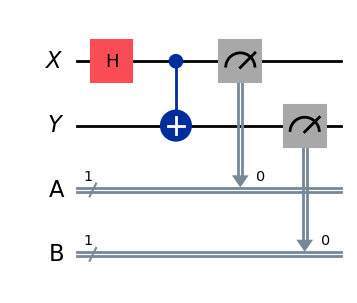
\includegraphics[width=0.85\linewidth]{pics/entangling.png}
        \caption{Entangling circuit}
        \label{fig:Entangling_circuit_A}
        \end{subfigure}%
        \begin{subfigure}{.5\textwidth}
        \centering
        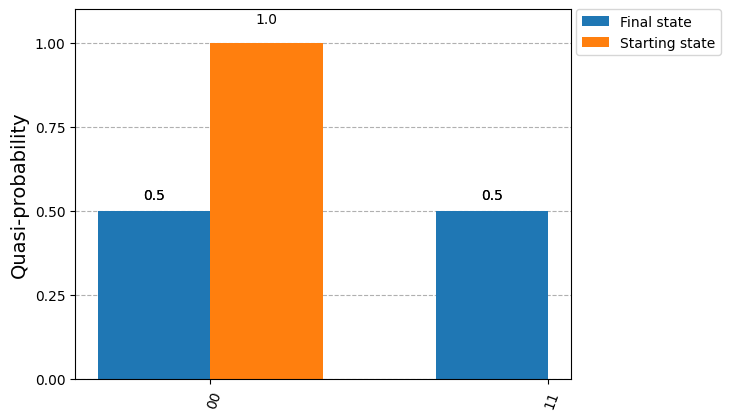
\includegraphics[width=1\linewidth]{pics/entangling_results.png}
        \caption{Result of circuit measurement}
        \label{fig:Entangling_circuit_B}
        \end{subfigure}
        \caption{$X$ and $Y$ denote the quantum bits, which we wil refer as variable qubits. 
        $A$ and $B$ are the classical registers, which we project our measurement results to. 
        The variable qubits posess the state $\ket{0}$, as seen in the orange histograms in \ref{fig:Entangling_circuit_B} 
        The gates are a Hadamard gate ($red$), and a Controlled-NOT ($blue$). The circuit results in $\hat{U}\ket{00} = C\hat{X}_{XY}\hat{H}_X\ket{00} = 
        C\hat{X}_{XY}\frac{1}{\sqrt{2}}(\ket{00} + \ket{10}) = \frac{1}{\sqrt{2}}(\ket{00} + \ket{11})$, which is depicted in the same subfigure as the starting state distibution, but 
        via the blue histograms.}
        \label{fig:Entangling_circuit}
        \end{figure}

        The action of a circuit on an initial state $\ket{\psi_0}$ is a sequence of unitary transformations:
        \[
        \ket{\psi_{\text{final}}} = U_k \cdots U_2 U_1 \ket{\psi_0},
        \]
        where each $U_i$ is a quantum gate.

        \subsection{Measurement in Quantum Mechanics}

        A measurement is the testing or manipulation of a physical system to yield a numerical result. In quantum mechanics it is when 
        a quantum state collapses to a classical outcome.
        Given an observable $\hat{O}$ we can write the spectral decomposition as:
        \begin{equation*}
            \hat{O} = \sum_i o_i \mathbb{P}_i
        \end{equation*}
        where $o_i$ are real numbers and $\mathbb{P}_i$ are projection operators to the eigenspace corresponding to the eigenvalue $o_i$. 
        
        Given a state $\rho$, when we measure the observable $\hat{O}$, we obtain one of its eigenvalues $o_i$ as an outcome.
        The probability $p_i$ and the state after measurement $\rho_i$ are:
        \begin{align*}
            p_i &= Tr(\mathbb{P}_i \rho)
            \\
            \rho_i &= \frac{1}{p_i}\mathbb{P}_i \rho \mathbb{P}_i
        \end{align*}

        For multi-qubit systems, measurement projects the state onto one of the basis vectors $\ket{k}$, with probability $|v_k|^2$. 
        \\
        An easy example is the single qubit superposition state from eq~\ref{eq:single_qubit_pure}:
        \begin{equation*}
            \rho = \ket{\psi}\bra{\psi} = \frac{1}{2}\begin{pmatrix}1 & 1 \\ 1 & 1 \\ \end{pmatrix}
        \end{equation*}
        and the Pauli-Z as an observable ($\hat{O} = \hat{Z}$), admitting to the spectral decomposition:
        \begin{equation*}
            \hat{O} = \hat{Z} = \begin{pmatrix}1 & 0 \\ 0 & 1 \\ \end{pmatrix} = o_0 \mathbb{P}_0 + o_1 \mathbb{P}_1
            = 1 \cdot \begin{pmatrix}1 & 0 \\ 0 & 0 \\ \end{pmatrix} + 1 \cdot \begin{pmatrix}0 & 0 \\ 0 & 1 \\ \end{pmatrix}
        \end{equation*}
        Thus when we measure the projector $\mathbb{P}_0$:
        \begin{align*}
            p_0 &= Tr(\mathbb{P}_0 \rho) = \frac{1}{2} Tr \begin{pmatrix}1 & 0 \\ 0 & 0 \\ \end{pmatrix} \begin{pmatrix}1 & 1 \\ 1 & 1 \\ \end{pmatrix} = \frac{1}{2}
            \\
            \rho_0 &= \frac{1}{p_0}\mathbb{P}_0 \rho \mathbb{P}_0 = 2 \cdot \begin{pmatrix}1 & 0 \\ 0 & 0 \\ \end{pmatrix} \frac{1}{2} \begin{pmatrix}1 & 1 \\ 1 & 1 \\ \end{pmatrix} 
            \begin{pmatrix}1 & 0 \\ 0 & 0 \\ \end{pmatrix} = \begin{pmatrix}1 & 0 \\ 0 & 0 \\ \end{pmatrix}
        \end{align*}
        and the projector $\mathbb{P}_1:$
        \begin{align*}
            p_1 &= Tr(\mathbb{P}_1 \rho) = \frac{1}{2} Tr \begin{pmatrix}0 & 0 \\ 0 & 1 \\ \end{pmatrix} \begin{pmatrix}1 & 1 \\ 1 & 1 \\ \end{pmatrix} = \frac{1}{2}
            \\
            \rho_0 &= \frac{1}{p_0}\mathbb{P}_0 \rho \mathbb{P}_0 = 2 \cdot \begin{pmatrix}0 & 0 \\ 0 & 1 \\ \end{pmatrix} \frac{1}{2} \begin{pmatrix}1 & 1 \\ 1 & 1 \\ \end{pmatrix} 
            \begin{pmatrix}0 & 0 \\ 0 & 1 \\ \end{pmatrix} = \begin{pmatrix}0 & 0 \\ 0 & 1 \\ \end{pmatrix}
        \end{align*}

        The outcome is inherently probabilistic, a fundamental departure from classical computation.

        \paragraph{Entanglement and Measurement:}
        Measurement on one qubit of an entangled pair instantaneously determines the outcome of the other, a phenomenon with no classical 
        analog. For example, measuring one qubit of the Bell state $(\ket{00} + \ket{11})/\sqrt{2}$ collapses the other qubit to the 
        same value, with causality being preserved, since no information is being transmitted during the measurement process 
        (which is called the no communication theorem~\cite{No_comm_theor}).
        It will be utilized in my implementation to enable backpropagation as a learning procedure.

    \section{Amplitude Amplification: Theory and Practice}
    \label{sect:QSA_AA}
    Amplitude amplification is a quantum algorithmic technique that generalizes Grover's search~\cite{Grover}, providing a quadratic 
    speedup for the identification or sampling of target states in an unstructured search space. The power of amplitude 
    amplification lies in its ability to systematically increase the probability amplitude associated with desirable outcomes, 
    making it a central primitive for quantum-enhanced sampling in machine learning.

        \subsection{Grover’s Algorithm and Generalizations}

        Grover’s algorithm is the canonical example of amplitude amplification. In the classical setting, searching for a marked item in an 
        unsorted database of size $N$ requires, on average, $O(N)$ queries, as with random selection, each and every item would have a 
        $\frac{1}{N}$ probability of finding, Grover’s quantum approach reduces this to $O(\sqrt{N})$ by exploiting quantum superposition 
        and entanglement.

        The algorithm operates in an $N$-dimensional Hilbert space $\mathcal{H}$, where each basis state $\ket{k}$ encodes a possible 
        solution. A Boolean oracle function $\chi: \{0,1\}^n \rightarrow \{0,1\}$ identifies target states. The oracle operator $\mathbf{O}$ 
        applies a phase flip to these states, while the diffusion operator $\mathbf{D}$ amplifies their amplitudes.

        Brassard et al.~\cite{Brassard_2002} extended Grover’s idea to arbitrary initial states and general quantum algorithms, formalizing the amplitude amplification operator:
        \begin{equation*}
        \mathbf{Q} = -\mathcal{A} \mathbf{S}_0 \mathcal{A}^{-1} \mathbf{S}_\chi
        \end{equation*}
        where $\mathcal{A}$ prepares the initial state over $n$ qubits ($\ket{\psi} = \mathcal{A}\ket{0}^{\tens{}n}$), $\mathbf{S}_\chi$ flips the phase of good states, and $\mathbf{S}_0$ flips the phase of the all-zero state. Repeated 
        application of $\mathbf{Q}$ rotates the quantum state in the two-dimensional subspace spanned by the good and bad components, continuously increasing the probability 
        of measuring a good state.

        \subsection{Oracle and Diffusion Operator Design}

        The effectiveness of amplitude amplification hinges on the careful design of the oracle and diffusion operators.

        \paragraph{Oracle Operator $\mathbf{O}$:}
        The oracle is a unitary operator that marks the set of good states by flipping their phase. For a basis state $\ket{k}$, in the state space $\mathcal{S} := \{\ket{k}\}_{k=0}^{N-1}$,
        \begin{equation*}
        \mathbf{O} \ket{k} = (-1)^{\chi(k)} \ket{k}
        \end{equation*}
        where $\chi(k) = 1$ for good states and $0$ otherwise. In practical terms, the oracle is implemented as a quantum circuit that 
        evaluates the Boolean function $\chi$ and applies a controlled-$Z$ or multi-controlled Toffoli gate to flip the phase of the target states. 
        For simple logical connectives, such as AND or OR, the circuit construction is straightforward. For more complex constraints, the circuit 
        depth increases, but the principle remains the same: the oracle must be a reversible, unitary operation that encodes the solution set 
        into phase flips. Of course here we assume that we know what the \textit{target} state and our state space is, but with an unknown \textit{target},
        the procedure requires some help, in the form of either a sensing algorithm, or an additional ancilla on which a phase oracle can be applied, 
        but this will not be neccesary with our conditions.

        \paragraph{Diffusion Operator $\mathbf{D}$:}
        The diffusion operator, or “inversion about the mean,” amplifies the amplitudes of the marked states. For an initial state 
        $\ket{\psi} = \mathcal{A}\ket{0}$, the diffusion operator is
        \begin{equation*}
        \mathbf{D} = 2\ket{\psi}\bra{\psi} - \mathbb{1}
        \label{eq:diffusion}
        \end{equation*}
        This operator reflects the quantum state about the initial state vector. In the special case where $\ket{\psi}$ is the uniform superposition, $\mathbf{D}$ can be 
        implemented by Hadamard gates, a phase flip on $\ket{0}$, and another round of Hadamards. For non-uniform initial states, the diffusion operator is constructed by 
        applying the inverse of the state preparation circuit, a phase flip on $\ket{0}$, and then re-applying the state preparation.

        \paragraph{Geometric Interpretation:}
        The interplay between the oracle and diffusion operators can be visualized as a sequence of reflections in a two-dimensional subspace. 
        With a projection operator emerging from the definition of $\mathbf{O}$;\
        \begin{equation*}
            \mathcal{P} := \sum_{\chi(k) = 1} \ket{k}\bra{k}
        \end{equation*} 
        defining the good and bad subspaces respectively:
        \begin{align*}
            \mathcal{H}_G := Im(\mathcal{P}) = span\{ \ket{k} \in \mathcal{S}_{op} \; | \;\chi(k) = 1\}
            \\
            \mathcal{H}_B := Ker(\mathcal{P}) = span\{ \ket{k} \in \mathcal{S}_{op} \; | \;\chi(k) = 0\}
        \end{align*} 
        If we adopt the convention of $\sum'$ for summation over the solution states, and $\sum''$ for summation over the non-solutions, we can define normalized states as such:
        \begin{align*}
            \ket{x_G} = \sqrt{\frac{1}{M}} \sum'_x \ket{x} 
            \\
            \ket{x_B} = \sqrt{\frac{1}{N - M}} \sum''_x \ket{x}
        \end{align*}
        where \textbf{N} is the number of states ($2^n$ for n qubits) and \textbf{M} is the number of solution states. Thus the initial state can be realized as:
        \begin{equation*}
            \ket{\psi} = \sqrt{\frac{N - M}{N}} \ket{x_B} + \sqrt{\frac{M}{N}}\ket{x_G} = \cos\left( \frac{\alpha}{2} \right) \ket{x_B} + \sin\left( \frac{\alpha}{2} \right)\ket{x_G}
        \end{equation*} 
        This is then a two-dimensional subspace spanned by the vectors $\ket{x_G}$ and $\ket{x_B}$. It is closed under the action of $\mathbf{Q}$.
        The oracle reflects the state about the bad subspace (i.e. the $\ket{x_B}$ register), while the diffusion operator reflects about the initial state.

        The composition of these two reflections is a rotation by an angle of $\alpha$ towards the good subspace. This geometric process underlies 
        the quadratic speedup of amplitude amplification, which will be cleared in the next section, where coming from the geometric interpretation
        we can calulate the updated amplitude of our state with each rotation, therefore we are able to have a value for the number of rotations needed for 
        maximum amplification.


        \subsection{Parameter Update Interpretation}
        \label{subsect:QSA_AA_paramupdate}

        The action of the amplitude amplification operator $\mathbf{Q}$ can be interpreted as two reflections -- once over the bad states, 
        and then over the average amplitude of our states (i.e. the register itself in the two-dimensional subspace) -- which geometrically is a rotation in the 
        two-dimensional subspace of the Hilbert space spanned by the projections of the initial state onto the good and bad subspaces. The initial state can be 
        written as
        \begin{equation*}
        \ket{\psi} = \sin \left( \frac{\alpha}{2} \right)\ket{\psi_g} + \cos \left( \frac{\alpha}{2} \right)\ket{\psi_b}
        \end{equation*}
        where $\ket{\psi_g}$ and $\ket{\psi_b}$ are normalized projections onto the good and bad subspaces respectively, ultimately resulting in
        the 2 dimensional subspace, which I will refer to as $H_{\psi}$. 
        The result of said rotations in $H_{\psi}$ can be depicted as seen in figure~\ref{fig:Grover_rot_diag}.
        As the state is stable under the action of $\mathbf{Q}$, the rotaion angle of $\frac{\alpha}{2}$ is given. Thus, 
        Each application of $\mathbf{Q}$ rotates the state by $2\cdot \frac{\alpha}{2} = \alpha$, such that after $k$ iterations,
        \begin{equation*}
        \mathbf{Q}^k \ket{\psi} = \sin\left((2k+1)\frac{\alpha}{2} \right)\ket{\psi_g} + \cos\left((2k+1)\frac{\alpha}{2} \right)\ket{\psi_b}
        \end{equation*}
        
        The probability of measuring a good state thus increases quadratically with the number of iterations, reaching a maximum when $(2k+1)\frac{\alpha}{2} \approx \pi/2$,
        resulting in:
        \begin{equation}
            k = \lfloor \frac{\pi}{4}\sqrt{\frac{1}{P_g^0}} \rfloor
        \label{eq:needed_k}
        \end{equation}
        meaning, that after exactly $k$ rotations we will have a maximum amplification of our state. This repeated applications, each resulting in 
        a rotation with angle $\alpha$, can be seen in a 3-dimensional representation in figure~\ref{fig:Grover_rot_mine}, where the axes are the $bad$ ($\ket{\psi_b}$)
        and $good$ ($\ket{\psi_g}$) states, spanning $H_{\psi}$. It is also visible now, that compared to classical algorithms, that can reach a time-depth of 
        $\mathcal{O}(\frac{1}{P}) = \mathcal{O}(N)$, with amplitude amplification we are able to reach $\mathcal{O}(\sqrt{\frac{1}{P}}) = \mathcal{O}(\sqrt{N})$, which is a 
        quadratic speedup for quantum algorithms over classical.  

        \begin{figure}
        \centering
        \begin{subfigure}{.5\textwidth}
        \centering
        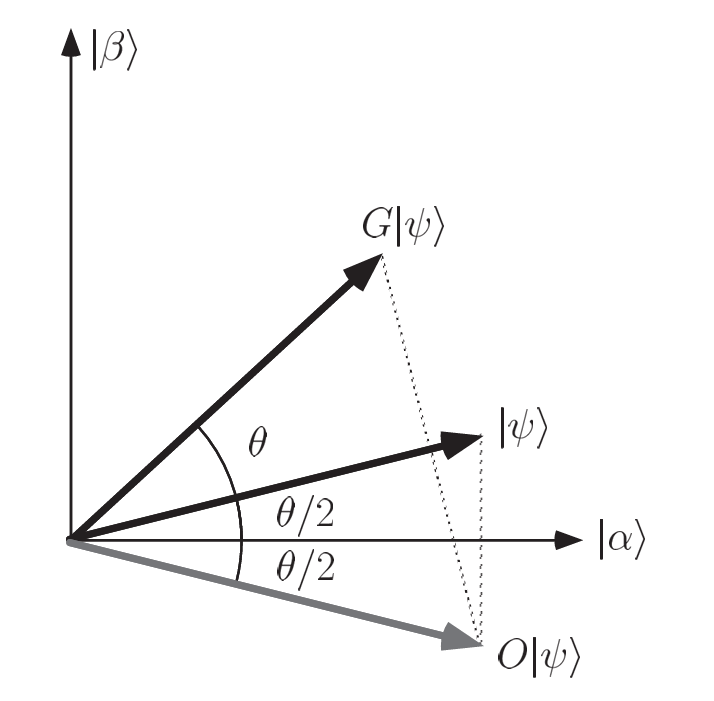
\includegraphics[width=\linewidth]{pics/grover_rot.png}
        \caption{Grover rotation in the 2 dimensional subspace $H_{\psi}$}
        \label{fig:Grover_rot_diag}
        \end{subfigure}%
        \begin{subfigure}{.5\textwidth}
        \centering
        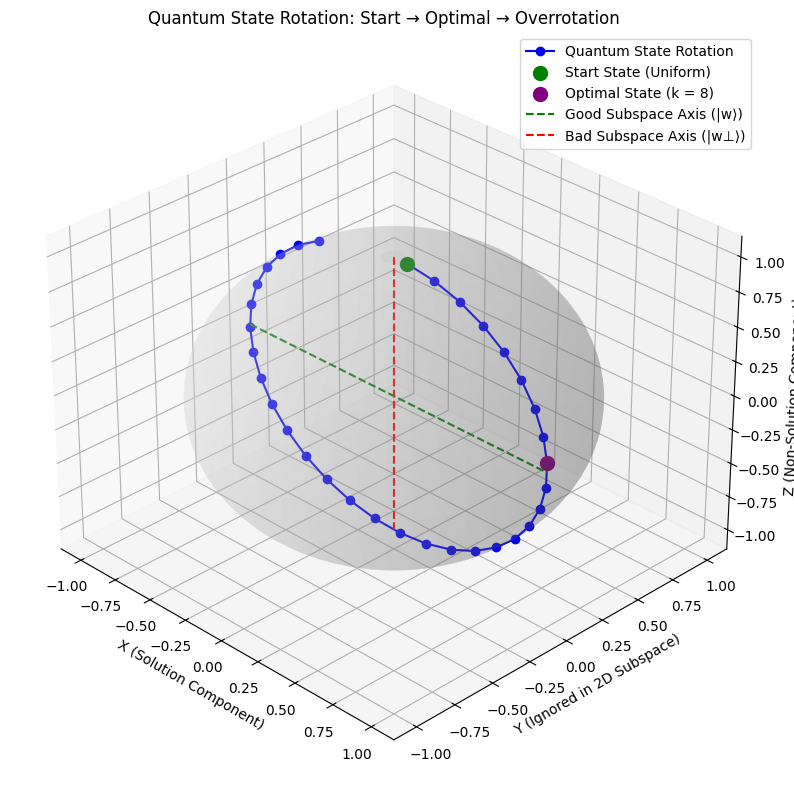
\includegraphics[width=\linewidth]{pics/Quantum State Rotation 3D.png}
        \caption{ Repeated applications in the complete state space}
        \label{fig:Grover_rot_mine}
        \end{subfigure}
        %\caption{Amplitude amplification bz repeated Grover rotations}
        \label{fig:Grover_rot}
        \end{figure}


        \subsection{Scalability and Simulator Limitations}
        The scalability of amplitude amplification is determined by the complexity of the oracle and diffusion operators, the number of required rotations $k$, 
        as well as the available quantum resources. For simple logical connectives and small models, both operators can be implemented with shallow 
        circuits, and the algorithm can be simulated efficiently on classical hardware. In this case allocating one qubit for each variable 
        (node), we have $n$ number of quantum registers, each followed by a constant number of gates representing the structure (i.e. the probabilities encode in amplitudes).
        Thus the state preparation can be done with a circuit of depth $\mathcal{O}(c_0 n)$, where $c_0$ represents the constant number of gates per variable qubit. 
        As we are working around binary valued variables we only need a simple gate sequence for the oracle ($\hat{Z}$ or $\hat{X}\hat{Z}\hat{X}$). The diffusion operator would 
        admit to the sequence $\mathcal{A}^{-1} CC\hat{Z} \mathcal{A}$. Thus $k$ rotations would result in a depth of $\mathcal{O}(k \cdot (2c_0n))$, where we dropped the 
        constant number of gates unrelated to n. Thus the whole process requires a circuit of depth $\mathcal{O}((1 + 2k) \cdot c_0 n)$
        which is $\approx \mathcal{O}(n + kn)$. Thus we have a state preparation of $\mathcal{O}(n)$ plus the amplification of $\mathcal{O}(kn)$.
        For more complex logical formulas or high-dimensional models, the circuit depth and qubit count increases. We need more ancillas for the structure encoding, and with more qubits, and 
        possibly lower probability for achieving the target, a higher number of Grover iterations would be needed. This means that inherently, more gates are involved in both the state preparation 
        and the amplification procedures. Therefore classical simulation becomes intractable.

        In this work, quantum simulations were performed for circuits up to 25 qubits using the Qiskit Aer simulator, balancing accuracy and 
        computational feasibility. For larger problem sizes, efficient simulation may require tensor network-based methods or access to real 
        quantum hardware. The quadratic speedup of amplitude amplification remains, but practical implementation is constrained by current 
        hardware and software limitations.
    
    \section{From Tensor Networks to Quantum Circuits}
    \label{sect:TN2Quantum}
        Tensor networks unify the representation of probabilistic models with quantum state encoding, as probabilistic models can be represented as such~\ref{subsect:Foundations_TN_ProbNetw},
        while quantum states - for example matrix product states (MPS) and projected entangled pair states (PEPS) - are inherently represented as tensor networks~\cite{TNforQC}.
        Therefore tensor networks provide a unified framework for representing and manipulating probabilistic models, as both probabilistic algorithms (e.g.inference),
        and quantum algorithms (such as Amplitude amplification) operate on these networks, providing a pathway to quantum-enhanced sampling.
        
        \subsection{Quantum Circuit Construction}
        \label{sect:TN2Quantum_construction}
            To map a tensor network to a quantum circuit, we need to map the intricate structure, involving connections and dependencies precisely.
            Slice tensor decomposition~\ref{subsect:Foundations_EXP2TN_slice} helps us decompose the given network to lower-rank tensors (1 and 2, i.e. 
            vectors and matrices representing state vectors and density operators), that can be mapped to quantum states and operations easily. 
            Thus each tensor (i.e. slice) can be encoded as a quantum state and/or a set of parameterized 
            quantum gates. The contraction of tensors, which in the classical setting corresponds to summing over shared indices, is implemented 
            in the quantum setting by entangling qubits or applying multi-qubit gates. For example, in a network where each variable $X_i$ 
            is binary, a qubit is allocated for each variable, and the entries of the tensor slices determine the amplitudes of basis 
            states, which can be applied as parameterized gate-sets.
        
        \newpage
        \textbf{Operational Steps:}

        \textbf{Decomposition}

            The joint probability tensor $\mathcal{T}[X_1, \ldots, X_n]$ for an $n$-variable exponential family distribution can be factorized as per~\ref{subsect:Foundations_EXP2TN_slice}: 
            \begin{align*}
                \mathcal{T}[X_1, \ldots, X_n] &= \sum_{k=1}^r \lambda_k \, \mathcal{A}_k[X_1] \otimes \mathcal{B}_k[X_2, \ldots, X_n]\\
                \intertext{or, more generally, as per~\ref{subsect:StepByStep}:}   
                \mathcal{T}[X_1, \ldots, X_n] &= \sum_{k=1}^r \mathcal{S}_k[X_1] \cdot \mathcal{U}_k[X_2] \cdots \mathcal{V}_k[X_n]
            \end{align*}
            where we have the tensor network uniqely decomposed into slices, ready to be represented as quantum states.

            This decomposition—closely related to the canonical polyadic (CP) decomposition, it maps naturally to quantum resources: 
            each vector or rank-1 slice defines amplitude weights for a subset of qubits, and higher-order correlations are encoded as 
            entanglement patterns or controlled gates.

        \textbf{Implementation}
            Integrating the above with the earlier sections, the practical quantum circuit mapping unfolds as:
            \begin{itemize}
                \item \textbf{State Preparation} $\mathcal{A}$: 
                    \begin{itemize}
                        \item Prepare the quantum register in a reference state (e.g., $\ket{0}^{\otimes n}$).
                        \item Apply Hadamard gates to all variable qubits, creating a uniform superposition over all $2^n$ states.
                        \item Use CNOT, Toffoli, and (optionally) parameterized rotation gates to encode the logical structure specified 
                        by the tensor network slices, projecting immeadiate nodes/results to designated ancilla qubits.
                    \end{itemize}
                \item \textbf{Oracle Construction} ($O_\phi$):
                    \begin{itemize}
                        \item Construct an oracle that flips the phase of those basis states corresponding to solutions (the "good" states satisfying $\phi$ of the exponential family). 
                        \item In practice, for logical connectives, this can be realized by targeted $Z$, $X$, or multi-controlled $Z$ gates operating on the 
                        ancilla qubit(s) where the satisfaction of $\phi$ has been projected.
                    \end{itemize}
                \item \textbf{Diffusion Operator} $D$:
                    \begin{itemize}
                        \item Apply the diffusion operator which inverts the state about the mean. This is constructed as applying $\mathcal{A}^{-1}$ (or $\mathcal{A}^+$), 
                        a phase flip on $\ket{0}^{\otimes n}$, and $\mathcal{A}$ again. Thus $D \propto \mathcal{A}^{-1} MC\hat{Z} \mathcal{A}$
                        \item Both $\mathcal{A}$ and its inverse are efficient to implement due to the decomposition structure, mirroring the original tensor slice encoding.
                    \end{itemize}
                \item \textbf{Amplitude Amplification}:
                    \begin{itemize}
                        \item Iteratively apply $Q = D O_\phi$ to amplify the amplitude of the "good" state subspace.
                        \item The number of iterations $k$ is chosen according to the initial probability and the target amplification, as detailed in Section~\ref{subsect:QSA_AA_paramupdate}.
                    \end{itemize}
                \item \textbf{Measurement:}
                    \begin{itemize}
                        \item Measure the final state in the computational basis.
                        \item Measure the variable qubits (i.e. the nodes of our tensor network) in the computational basis.
                    \end{itemize} 
            \end{itemize}

            By combining the slice decomposition approach (Section~\ref{subsect:Foundations_EXP2TN_slice}) with tensor-to-circuit 
            compilation presented in this section, this quantum circuit implementation provides a systematic bridge from classical 
            probabilistic and logical models to quantum-enhanced sampling routines. Each step - from state preparation using decomposed 
            tensor slices, to phase-marked oracles, to efficient inversion about the mean—follows directly from the underlying structure 
            revealed by the slice tensor decomposition. This guarantees scalability and resource efficiency for a wide range of complex probabilistic models.

            \begin{tcolorbox}[breakable, width=\linewidth, sharp corners=all, colback=white!95!black]
                Therefore utilizing the slice tensor decomposition we can map the example Bernoulli distribution to a quantum circuit easily.
                Each slice being jointly independent would mean that, we can not only encode them one-by-one, we do not even need to consider entangling gates/procedures.
                So for the distribution:
                \begin{equation*}
                P(x_1, x_2, \dots , x_n) = \prod_{i = 1}^n p_i^{x_i}(1-p_i)^{1-x_i}
                \end{equation*}
                we can encode each slice $p_i^{x_i}(1-p_i)^{1-x_i}$ to a quantum circuit via a sequence of gates, such as:
                \begin{itemize}
                    \item Generate a register for each variable, 1 for each slice.
                    \item Apply Hadamard gate $\hat{\textbf{H}}$ to create superposition.
                    \item Apply rotation gate around the $X$ or $Y$ axes ($\hat{\mathbf{R}}_X$ or $\hat{\mathbf{R}}_Y$) to encode the probabilities of the distribution resulting in $1$ or $0$, 
                    in the amplitude of the quantum state, i.e. mirroring the state resulting in $\ket{1}$ or $\ket{0}$ upon measurement.
                \end{itemize}
                Thus when we measure the circuit it should obtain one of the states representing the result of the measurement ($\ket{1}$ or $\ket{0}$), each with a probability
                that represents the distribution itself, obtained through the amplitude of the state. Also with a rotation applied to a superposition the state
                remains pure, so the probabilities will sum up to one.
                \\
                The amplitude amplification can be done for each slice via an easily applicable oracle and diffusion operator:
                \begin{itemize}
                    \item as we are working around binary variables a single $\hat{\textbf{Z}}$ or $\hat{\textbf{X}}\hat{\textbf{Z}}\hat{\textbf{X}}$ gate(set) would suffice to mark the 
                    $\ket{1}$ and $\ket{0}$ states respectively,
                    \item the diffusion opreator should consist of the inverse state preparation unitary $\mathcal{A}^{-1}$, and a single $\hat{\textbf{X}}$
                    gate to rotate around the mean amplitude of our starting state (esentially flipping $\ket{0}$ to $\ket{1}$).
                    \item Finally $\mathcal{A} \propto \hat{\textbf{H}}\hat{\mathbf{R}}_X$ could be applied again on all variable qubits, and we will get an amplified probability 
                    of obtaining $\ket{0}$ or $\ket{1}$ (depending on the Oracle).
                \end{itemize}
            \end{tcolorbox}

        \subsection{Resource Estimates}
            The quantum circuit depth and resource requirements depend on the structure and rank of the underlying tensor network:
            \begin{itemize}
                \item \textbf{Qubit Count}: Each variable in the model typically requires one qubit for binary variables (or 
                $\lceil \log_2 d_i \rceil$ qubits for $d_i$-ary variables) as well as one auxiliary qubit (i.e. ancilla qubit) for connecting the 
                cliques of probabilistic model representations~\ref{subsect:Foundations_TN_ProbNetw}.
                \item \textbf{Gate Complexity}: The number of gates scales with the number of tensor slices and the connectivity of the network. 
                For a CP decomposition of rank $r$ over $n$ variables, the circuit requires $\mathcal{O}(rn)$ parameterized gates~\cite{CPdecomp}.
                \item \textbf{Circuit Depth}: For chain-like (MPS) or tree-like (TTN) tensor networks, the depth is $\mathcal{O}(n)$ or $\mathcal{O}(\log n)$, respectively.
                %\item \textbf{Noise Considerations}: Shallow circuits and sparse connectivity are advantageous for near-term quantum devices, as they minimize decoherence and gate errors.
            \end{itemize}

            \begin{tcolorbox}[breakable, width=\linewidth, sharp corners=all, colback=white!95!black]
                As we have seen in the example mapping above we did:
                \begin{itemize}
                    \item require 1 qubit for each binary variable ($X_k \in \{X_1, X_2, \dots, X_n\}$),
                    \item as well as 1 Hadamard and 1 rotation gate for the probability encodings. So the state preparation can be done with $\mathcal{O}(2n)$ gates, where n is the number of variables.
                    \item Additionally each slice requires a constant number of gates for the amplitude amplification procedure, which then for k rounds is $\approx \mathcal{O}(k \cdot 2n)$.
                    \item Thus for N variables, the whole procedure results in a depth of $\approx \mathcal{O}(kn)$.
                    Therefore the number of gates scale with the number of tensor slices. In the case of the example (with joint independence between the variables)
                    it does scale linearly. The linear scaling of the state preparation matches the classical state preparation algorithms~\cite{APXML2025}. The $\mathcal{O}(k)$ scaling
                    of the sampling algorithm on the other hand is quadratically faster than the classical counterparts.
                \end{itemize}
            \end{tcolorbox}
            We can see that the mapping is particularly efficient when the tensor network has low rank or sparse structure, as is often the case for 
            models with strong conditional independence. In such scenarios, the number of required gates and the circuit depth can be kept 
            polynomial in the number of variables, making the approach feasible for near-term quantum devices~\cite{Ran_2020}.

            In summary, the mapping from exponential family distributions to tensor networks, and subsequently to quantum circuits, enables scalable quantum sampling for complex probabilistic models, 
            as seen by the application of amplitude amplification later on. This approach exploits both the structure of the underlying model and the computational power of quantum devices, providing 
            a pathway to quantum advantage in probabilistic inference and machine learning.

%\section{Noise and Error Modeling}

%\subsection{Effect of Noise on Quantum Sampling}

%Quantum circuits are inherently sensitive to noise and decoherence, which can degrade the fidelity of amplitude amplification and reduce the probability of successfully measuring a good state. Common noise sources include gate errors, measurement errors, and qubit decoherence. Simulations incorporating realistic noise models show that amplitude amplification remains effective up to certain noise thresholds, but error accumulation can significantly impact performance for deeper circuits or larger systems. Understanding these effects is crucial for designing error-resilient circuits and for resource estimation on near-term quantum devices.


\chapter{Experimental Evaluation}
\label{chapter:4}

Our goal in this section is to show the feasibility of the quantum sampling procedure promoted in the previous sections. It should be done by working through a 
dummy knowledge base, one chosen from the used instances in AI, previously collected in sect.~\ref{sect:Foundations_modelling}. After chosing a suitable subject
it will be represented as an exponential family, over which slice tensor decomposition will be utilized, so that the now sliced knowledge base can be mapped to a 
quantum circuit. Each variable will therefore be represented as a qubit, with the logical connections as quantum gates, within each slice, iteratively building the
dummy knowledge base, which is the logical formula. Then the sampling procedure will be tested, with the amplitude amplification involved. We will check the probabilities 
before and after sampling, to see how the $target$ state probabilities have been amplified. After this, it should clearly be visible that a quantum enhanced sampling procedure
can be utilized on classical knowledge bases, through a robust decomposition and mapping formalism.

    \section{Use Case: Logical Connective Sampling}            
        A logical formula is the representative knowledge base for testing the quantum sampling procedure. It has been chosen as the suitable subject 
        for testing, as we have been working around the \textbf{TNReason} module of sampling for neuro-symbolic AI, which predominantly utilizes 
        logical formulas as knowledge bases. This way we will not only test the quantum sampling procedure, but also see if it is implementable
        to the module we are working in. And if our experimental findings agree with the theory, it will be implemented as a baseline for future 
        quantum samplers, and possibly be utilized around financial datasets.

        \subsection{Problem Setup}
        \label{subsect:EE_Setup}

            The problem is defined as follows: given a logical formula \textbf{F} ($n$ Boolean variables connected by propositional logical connectives), our 
            goal is to sample satisfying assignments (\textit{target} states) from the exponentially large space of all $2^n$ possible assignments.
            For concreteness, let us focus on a n-qubit system encoding a logical connective such as seen in the previous example~\ref{eq:Logical_conn_ex}, 
            which for the sake of the example will be 6 variables (mapped to qubits), with 19 connectives, each represented as an ancilla qubit. 
            Therefore the whole quantum circuit requires 25 qubits. The set of \textit{target} states, $\mathcal{G}$, consists of all assignments that 
            satisfy the formula. The initial probability of selecting a good state from the uniform distribution is $P_g = M/N = |\mathcal{G}|/2^n$. 
            In the case of the example shown it equals $P_g = M/N = 1/2^6$, as we have $M=1$ good state, making that our $target$.
            Our aim is to amplify $P_g$ to near-unity using quantum amplitude amplification.

        \subsection{Exponential family representation of the Logical Formula}
        \label{subsect:EE_expfam_repr}
            The logical formula \textbf{F} can be encoded as an exponential family distribution as per~\ref{eq:expfam_def}:
            \begin{equation*}
                p(x) = \exp \{ \langle \theta , \phi(x) \rangle - A(\theta) \}
            \end{equation*}
            Serving as the sufficient statistics for the exponential family is $\hat{\mathbb{1}}[\textbf{F}]$, the indicator function for 
            the formula. $\theta$ is the (unnormalized) vector of the canonical parameters, showing the effect of the sufficient statistics as it has been deduced in 
            sect.~\ref{subsect:Foundations_ExpFam_Definition}.
            This value for $\theta$ in our case is:
            \begin{equation*}
                \theta = \begin{pmatrix}
                    \theta_g \\
                    \theta_b 
                \end{pmatrix}
            \end{equation*}
            which for $\theta_g$ and $\theta_b$ is:
            \begin{itemize}
                \item zero, whenever the indicator function gives a result of `FALSE'/0
                \item $\infty$, whenever it is `TRUE'/1
            \end{itemize}
            Using this representation, $\theta$ can be understood as the weight of the truth value of the formulas, coming directly from the sufficient 
            statistics being the indicator function of the logical formula. The log-partition function `$\mathit{\exp(- A(\theta))}$' can be rewritten with $Z$,
            serving as the normalization constant.
            \\
            Thus the exponential family is
            \begin{equation}
                p(x) = \frac{1}{Z} \exp\left\{ \theta \cdot \hat{\mathbb{1}}[\textbf{F}] \right\}
                \label{eq:log_exp_fam}
            \end{equation}
            
            Using this representation of the indicator function and canonical parameters as weights, we get probabilities:
            \begin{itemize}
                \item $p(x = 1) = \frac{Me^{\theta_g}}{(N - M)e^{\theta_b} + Me^{\theta_g}} = P_g$ 
                \item $p(x = 0) = \frac{(N-M)e^{\theta_b}}{(N - M)e^{\theta_b} + Me^{\theta_g}} = P_b$
            \end{itemize}
            with $N = 2^n$ as all the possible states, $M$ of which are \textit{target} states. Being a $target$ state means the indicator function resulting in 1!
            This gives a great starting point for us, as for both the `good' and `bad' states, wether $\theta=0$ this reduces to the uniform distribution; and as $\theta \to \infty$, $P \to 1$
            and the distribution concentrates on the satisfying assignments. Thus the expectation is this, that when the logical formula is mapped
            to a quantum circuit, an uniform distribution of variables is given, where all the outcomes (i.e. final states) have the same probability of $\frac{1}{N}$. 
            And when the probability of the \textit{target} states are amplified, only the canonical parameter of the formula will change, as it will diverge to infinite 
            values ($lim_{\theta \rightarrow \infty}(e^{\theta}) = \infty$). The sufficient statistics however, should remain
            the same, esentially keeping us in the same exponential family with tuned variables, to match our amplified quantum states.
            \\
            Then we need to apply slice decomposition on the defined exponential family to map each logical connection to the quantum circuit at hand.
            Following the definition in section~\ref{subsect:Foundations_EXP2TN_slice} we can slice the logical formula by each connective, thus making it straightforward
            to iteratively have every detail embedded into our initial state $\ket{\psi}$, prepared by the unitary $\mathcal{A}$, the direct result of the decomposition.

        \subsection{Amplitude Amplification for Exponential Families}
        When the locical formula is mapped to a quantum circuit, we start from a uniform distribution of variables, and slowly amplify 
        the probability of the \textit{target} states, thus changing the probability of finding such.

        Our expectation, and goal to prove, is that only the canonical parameter of the formula will change, whilst the sufficient statistics should remain
        the same. As when the amplitude of the \textit{target} states are amplified, the probabilities are magnified. Thus as per the definition
        for the exponential family in eq.~\ref{eq:log_exp_fam}, $\theta_g$ will diverge to infinite values. This way the procedure is esentially keeping us in 
        the same exponential family with finely tuned variables, to match the amplified quantum states.
        
        Mathematically, if the initial probability of a good state is $P_{g}^0$, then after $k$ applications of amplitude amplification, the probability becomes $P_g^k = \sin^2\left((2k+1)\frac{\alpha}{2}\right)$, 
        where $\frac{\alpha}{2} = \arcsin(\sqrt{P_{g}^0})$, is the angle of the state in $H_{\psi}$. In exponential family terms, this corresponds to a shift in the canonical parameter:
        \begin{align}
            \theta_g^k &= \ln\left(\frac{(1-P_{g}^0)P_g^k}{P_{g}^0(1-P_g^k)}\right) \\
            \intertext{which can be rewritten as:}
            \theta_g^k &= \ln \left( \frac{P_g^k}{1 - P_g^k} \right) - \ln \left( \frac{P_{g}^0}{1 - P_{g}^0} \right)
            \label{eq:Can_par_change}
        \end{align}
        So the canonical parameter for the $target$ states $\theta_g^k$ could be obtained as the the difference of log-odds (i.e. \textit{logit}, the inverse of the \textit{sigmoid}) between the current probability $P_g^k$ (the probability after $k$ rounds of amplification),
        and the initial probability $P_{g}^0$.

        This provides a direct link between quantum amplitude amplification and classical parameter updates in probabilistic models.

            \iffalse
            \begin{figure}[h]
                \centering
                \includegraphics[width=0.7\textwidth]{quantum_circuit_example.pdf}
                \caption{Quantum circuit implementing amplitude amplification for a 6-qubit logical connective. The oracle marks \textit{target} 
                states, and the diffusion operator amplifies their amplitudes.}
                \label{fig:aa_circuit}
            \end{figure}
            \fi

        \subsection{Quantum Circuit Implementation}
            The mapping from an exponential family model to a quantum circuit uses the slice decomposition of its tensor 
            network representation. This operational workflow links the mathematical structure of probabilistic graphical models 
            directly to the physical implementation of quantum sampling algorithms. The explicit role of slice tensor decomposition 
            is to enable a direct, scalable quantum encoding of the high-dimensional probability distribution, efficiently reflecting 
            its conditional independence structure and logical symmetries.

            In this section, I am illustrating how a specific logical formula is mapped to a quantum circuit using the slice tensor 
            decomposition of its exponential family representation.

            Given a logical formula \textbf{F} first defined in sect~\ref{subsect:EE_Setup}, and represented as an exponential family distribution in sect.~\ref{subsect:EE_expfam_repr}:
            \begin{equation*}
                p(x) = \frac{1}{Z} \exp\left\{ \theta \cdot \hat{\mathbb{1}}[\textbf{F}] \right\}
            \end{equation*}
            where, just like in eq.~\ref{eq:log_exp_fam}, $\hat{\mathbb{1}}[\textbf{F}]$ is the indicator function for the formula \textbf{F} - i.e. the sufficient statistics of the 
            exponential family, whilst $\theta$ is the canonical parameter, and $Z$ is the normalization constant.
            
        To map this to a quantum circuit, we are following the previously outlined construction and amplification schemes from sect.~\ref{sect:TN2Quantum_construction}:
        \begin{enumerate}
            \item \textbf{Slice Tensor Decomposition}: The indicator function $\hat{\mathbb{1}}[\textbf{F}]$ naturally partitions the joint tensor representing the distribution into two 
            slices—one for satisfying ("good") and one for non-satisfying ("bad") assignments. Mathematically, the joint distribution tensor is decomposed as:
            \[
            T[x] = \theta_g \cdot \hat{\mathbb{1}}[\textbf{F} = 1] + \theta_b \cdot \hat{\mathbb{1}}[\textbf{F} = 0]
            \]
            where the coefficients of the canonical parameter vector reflect the weights in the exponential family, as defined in sect.~\ref{subsect:EE_expfam_repr}.
            Both $\theta_g$ and $\theta_b$ start off as 0, thus for the probabilities we have:
            \begin{align*}
                p(x = 1) &= \frac{Me^{\theta_g}}{(N - M)e^{\theta_b} + Me^{\theta_g}} = P_g = \frac{M}{N}   \\
                p(x = 0) &= \frac{(N-M)e^{\theta_b}}{(N - M)e^{\theta_b} + Me^{\theta_g}} = P_b = \frac{N-M}{N}
            \end{align*}
            As with the logical formula mapped mapped as a quantum state, we should have an uniform superposition of variables, i.e. equal probabilities for all $N$ states, $P_i = \frac{1}{N}$. 
            \item \textbf{Quantum State Preparation}: The logical formula is compiled into a quantum circuit using ancilla qubits. Apply Hadamard gates to all variable qubits to create a 
            uniform superposition over all $2^n$ possible inputs, then use Toffoli and controlled gates to compute the value of $F(x)$ onto an final ancilla qubit. This then represents the whole formula, 
            so it will be called the \textit{indicator qubit}.
            \item \textbf{Oracle Marking}: A $Z$ gate (phase flip) is applied to the ancilla qubit, conditionally marking the satisfying assignments. 
            This realizes the "slice selection" from the tensor decomposition within the quantum circuit.
            \item \textbf{Diffusion and Amplitude Amplification}: The standard amplitude amplification procedure is then applied, increasing the probability amplitude on the "good" slice. 
            After the desired number of amplification rounds, measurement yields satisfying assignments with high probability, while the underlying tensor slice structure ensures the 
            exponential family is preserved with an updated parameter $\theta$.
        \end{enumerate}
        The pseudocodes for the test example can be seen in the Appendix~\ref{Appendix_pseudocodes}.
        In summary, this process implements the slice decomposition of the exponential family for a logical formula as a natural quantum circuit: logical structure—encoded as tensor 
        slices—is mapped onto programmable quantum operations and oracles, efficiently targeting the satisfying assignments for sampling and inference.

        \section{Results and Analysis}
        \label{sect:EE_Results}
            After $k$ rounds of amplitude amplification, the probability of measuring a good state increases from $P_g^0$ to $P_g^k = \sin^2((2k + 1)\alpha)$.
            Deduced from the starting probability for a \textit{target} state, $\alpha = \arcsin(\sqrt{P_g^0})$.
            The canonical parameter of the exponential family updates as seen in eq~\ref{eq:Can_par_change}.

            The changes in probabilities of the given logical formula can be seen in the following figures:

            \begin{figure}[H]
            \centering

            \begin{subfigure}{\textwidth}
            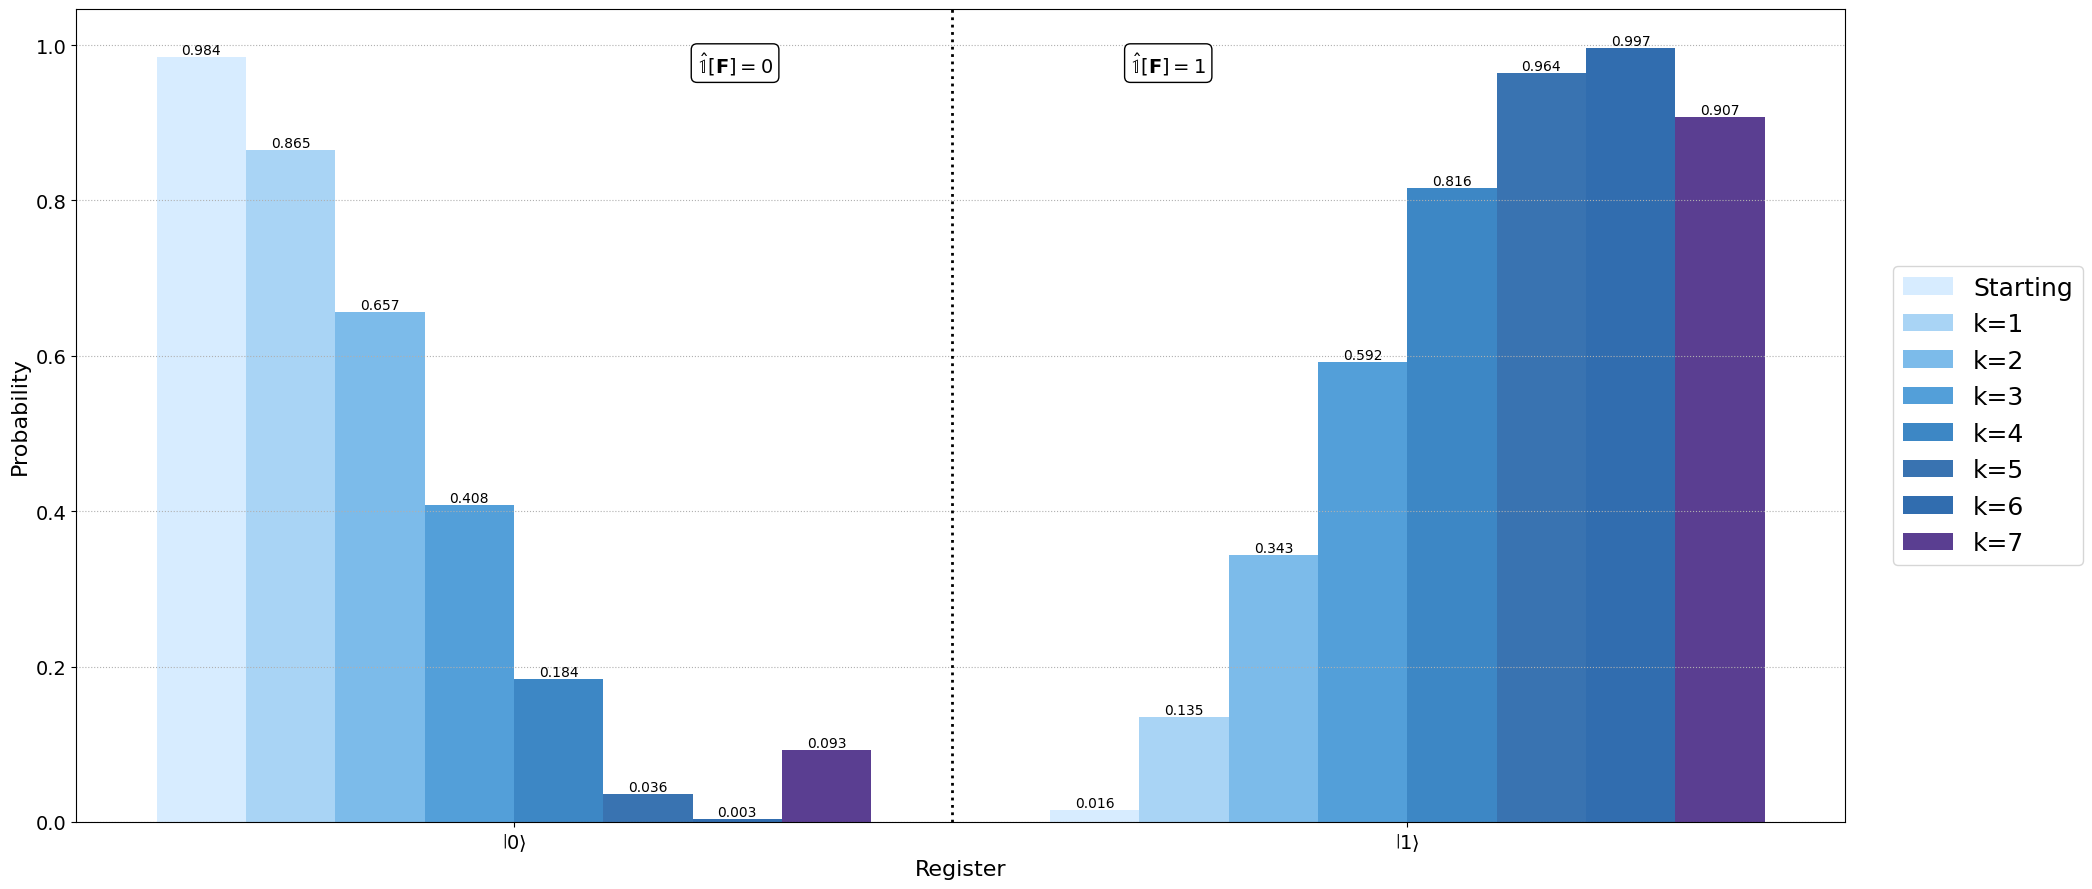
\includegraphics[width=\linewidth]{pics/overrotation_final6.png}
            \caption{Probability $P_{g}$ of measuring TRUE/FALSE value on the logical formula, indicated by the value of the \textit{indicator qubit} }
            \label{subfig:AA_final}
            \end{subfigure}

            \medskip % insert a bit of vertical whitespace
            \begin{subfigure}{\textwidth}
            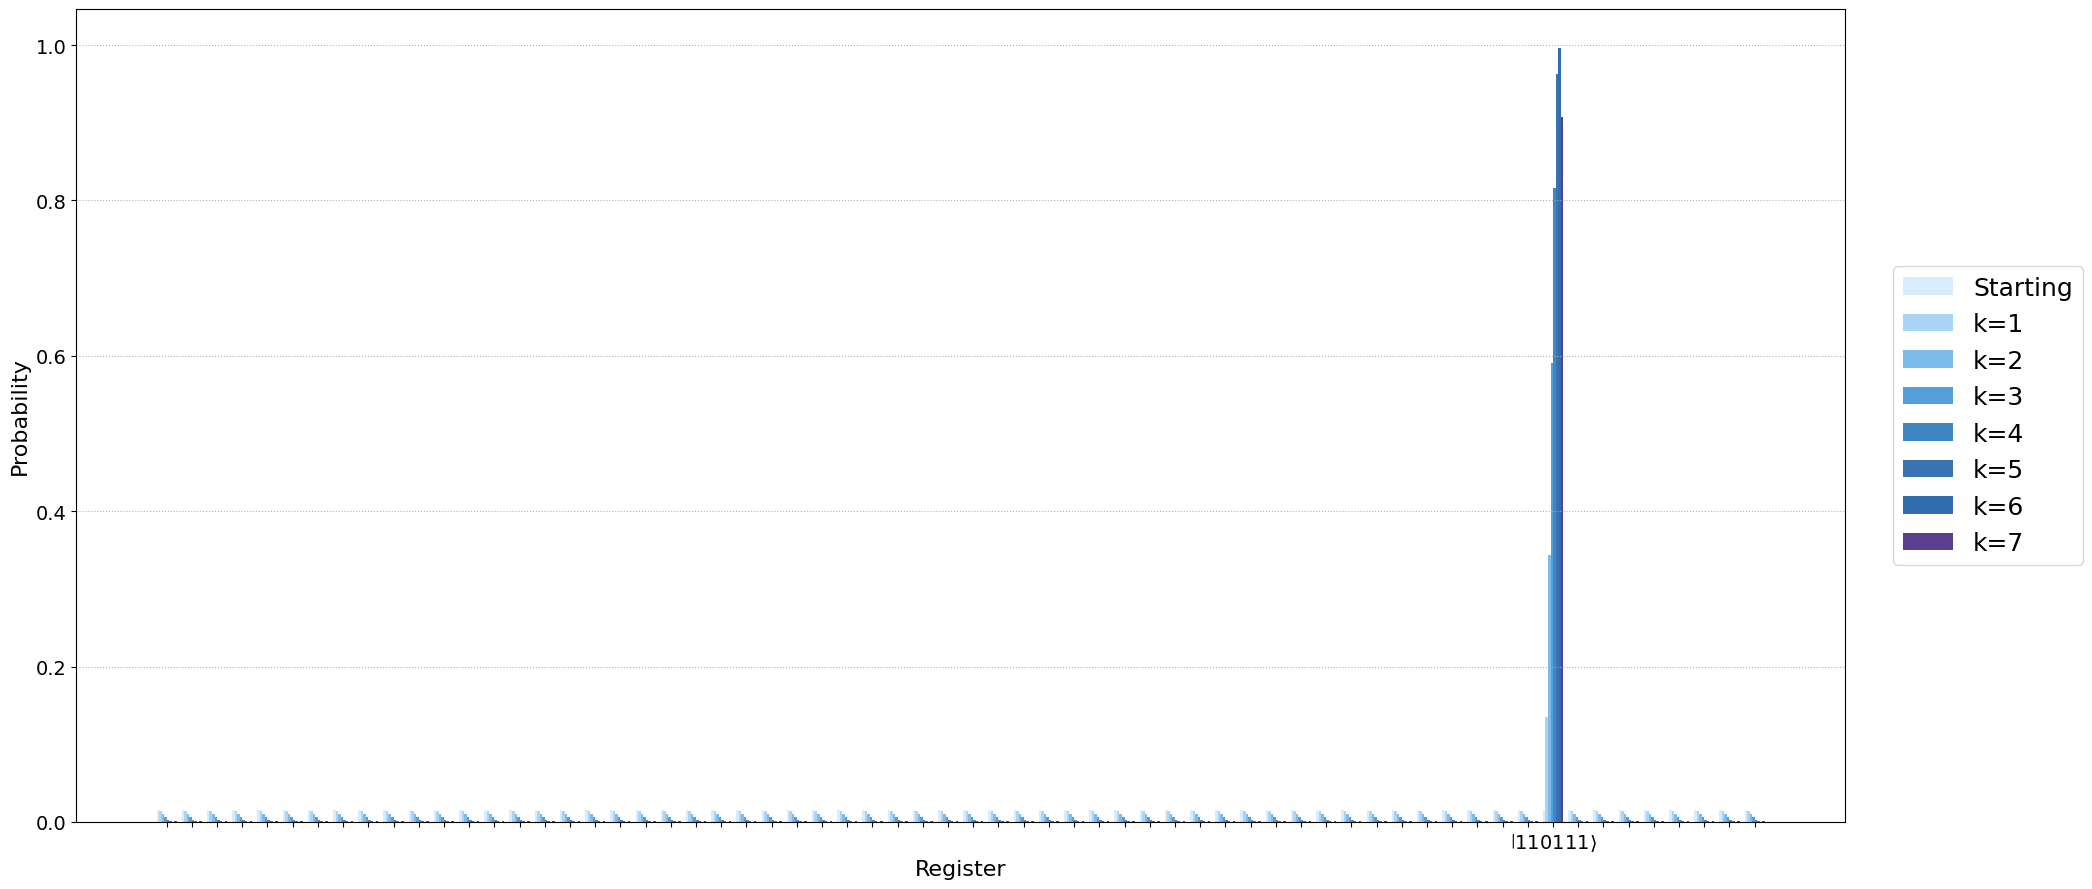
\includegraphics[width=\linewidth]{pics/overrotation_variable6.png}
            \caption{Probabilities of the variable qubit values. The \textit{target} state is visible, it will result in the value of the \textit{indicator qubit} being 1}
            \label{subfig:AA_variable}
            \end{subfigure}

            \caption{Changing \textit{indicator qubit} and variable qubit state probabilities after $k$ iterations of Grover rotations on a given logical formula $\textbf{F}$.}
            \label{fig:AA_log_formula}

            \end{figure}

            We can see that we have achieved near perfect amplification after 6 steps, which is in agreement with the theory presented in sect.~\ref{subsect:QSA_AA_paramupdate},
            that $k = \lfloor \frac{\pi}{4}\sqrt{\frac{1}{P_g}} \rfloor = \lfloor \frac{\pi}{4}\sqrt{\frac{64}{1}} \rfloor = 6$. The seventh step, as expected,
            lowers the success probability, meaning that we have overrotated. This overrotation in on par with our calculations for the graphical interpretation
            of the parameters in sect.~\ref{subsect:QSA_AA_paramupdate}.

            The corresponding changes angle, probabilities and $\theta_k$ are:

            \begin{table}[H]
                \centering
                \begin{tabular}{|c|c|c|c|}
                    \hline
                    Iteration ($k$) & $P_g$ & $\alpha_k$ (rad) & $\theta_k$ \\
                    \hline
                    0 & $0.016$ & $0.126$ & $0$ \\
                    \hline
                    1 & $0.134$ & $0.375$ & $1.543$ \\
                    \hline
                    2 & $0.344$ & $0.626$ & $2.763$ \\
                    \hline
                    3 & $0.592$ & $0.878$ & $3.781$ \\
                    \hline
                    4 & $0.817$ & $1.129$ & $4.905$ \\
                    \hline
                    5 & $0.963$ & $1.378$ & $6.668$ \\
                    \hline
                    6 & $0.997$ & $1.516$ & $9.215$ \\
                    \hline
                    7 & $0.908$ & $1.263$ & $5.698$ \\
                    \hline
                \end{tabular}
                \caption{Amplification of probability and exponential family parameter over iterations.}
                \label{tab:amplification_results}
            \end{table}

            \noindent
            \textbf{Interpretation:} The amplitude amplification procedure efficiently concentrates probability mass on the set of 
            satisfying assignments. This was achieved under $\mathcal{O}(k)$ steps, preserving quadratic speedup over classical sampling 
            methods. The other important result is that the process preserves the exponential family structure of the distribution, with 
            the canonical parameter $\theta$ evolving according to the amplification dynamics shown in eq.~\ref{eq:Can_par_change}. 
            This demonstrates the compatibility of quantum amplitude amplification with classical probabilistic 
            modeling frameworks, showing the viability of the sampling approach.

    \subsection{Canonical Parameter Dynamics in Large-Scale Simulations}
    While the initial example demonstrated precise amplification behavior for a relatively small quantum circuit - comprising 6 variable qubits and 19 
    ancillary qubits; the following figures (\ref{fig:can_changes} and \ref{fig:can_gb_2}) do not stem from direct simulation of a larger circuit as with current hardware, classical simulation is intractable, 
    while consumer grade trapped-ion computers are not available for this large qubit numbers. Rather, they illustrate the theoretically calculated dynamics of the 
    angle, probability, and canonical parameters, extended to the regime of much smaller $target$ state probabilities and therefore a greater number of amplitude amplification rotations. This 
    approach reinforces the generality and robustness of the theoretical models presented earlier, and allows for a clearer depiction of amplitude dynamics and 
    the evolution of exponential family parameters under deep amplification sequences.

    \paragraph{Sinusoidal Variation of Sampling Probabilities}
    As we have seen previously in eq.~\ref{eq:Can_par_change}, the core mechanism underpinning amplitude amplification is a rotation in 
    the two-dimensional subspace of the state space - spanned by the “good” states (those satisfying the desired logical formula) and the “bad” states (non-satisfying). 
    The probability of measuring a “good” state after $k$ iterations is given by
    \begin{equation*}
        P_g^k = \sin^2\bigl((2k + 1) \frac{\alpha}{2}\bigr),
    \end{equation*}
    where $\alpha = \arcsin\sqrt{P_g^0}$ is related to the initial probability of the good states in the uniform superposition.

    The sinusoidal waveforms in the figures~\ref{fig:can_changes} vividly illustrate this fundamental oscillatory behavior: with each application of the amplification operator, 
    the likelihood of observing a target solution state upon measurement is periodically increased.
    It leads to an optimal number of iterations corresponding to the peak of the sinusoid. Beyond this point, further iterations induce overrotation, causing the probability 
    of success to decrease, as evidenced by the downturn observed in the latter part of the figure.

    \paragraph{Canonical Parameter Explosions and Their Interpretation}
    The canonical parameter $\theta$ associated with the canonical representation of the exponential family undergoes shifts in close ties with the 
    success probability $P_g^k$. The relationship ties the probability dynamics to changes in the distribution parameters via
    \begin{equation*}
        \theta_g^k = \ln \left( \frac{P_g^k}{1 - P_g^k} \right) - \ln \left( \frac{P_{g}^0}{1 - P_{g}^0} \right)
    \end{equation*}
    capturing the evolution of $\theta$ as a differential log-odds ratio between the amplified and initial state probabilities.

    The sinusoidal behavior of $P_g^k$ translates into a highly non-linear, even discontinuous, evolution of $\theta_g$. Near points where $P_g^k$ approaches unity or zero, 
    the canonical parameter exhibits steep, near-explosive growth, resembling the vertical asymptotes in the log-odds function. This shootout of $\theta_g$ effectively tightens the probability 
    mass around the solution set, pushing the distribution towards deterministic support on the satisfying states. The dynamics can be seen in figures \ref{fig:can_changes} compared to the sinusoidal
    change in probability, and in subfigure \ref{subfig:can_ANG_gb}, comparing the $\theta_g$ to $\theta_b$.

    \nopagebreak
    Such shifts in $\theta$, as being deductable from the probabilities and angles of the $target$ state, highlight the capabilities of the procedure.
    Quantum amplitude amplification increases success probabilities, thus also tunes the parameters of the underlying exponential family representation. In effect, this quantum sampling process updates 
    the distribution's parameters analogous to classical iterative parameter update schemes, yet achieves this transformation quadratically faster in the size of the state space.
            
            \begin{figure}[H]
            \centering

            \begin{subfigure}{0.65\textwidth}
            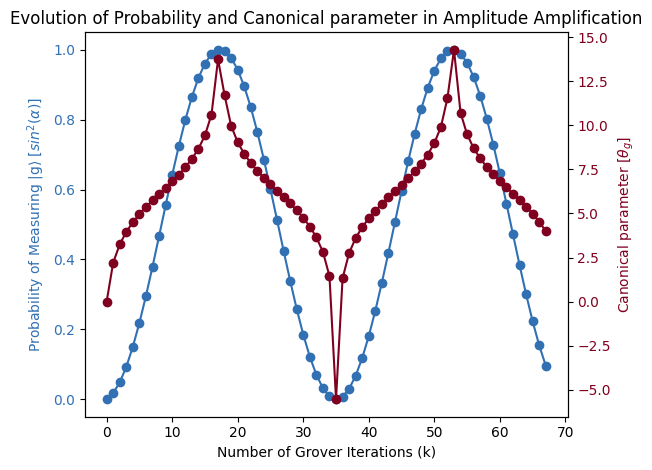
\includegraphics[width=\linewidth]{pics/can_prob.png}
            \label{subfig:can_PROB}
            \end{subfigure}

            \medskip % insert a bit of vertical whitespace
            \begin{subfigure}{0.75\textwidth}
            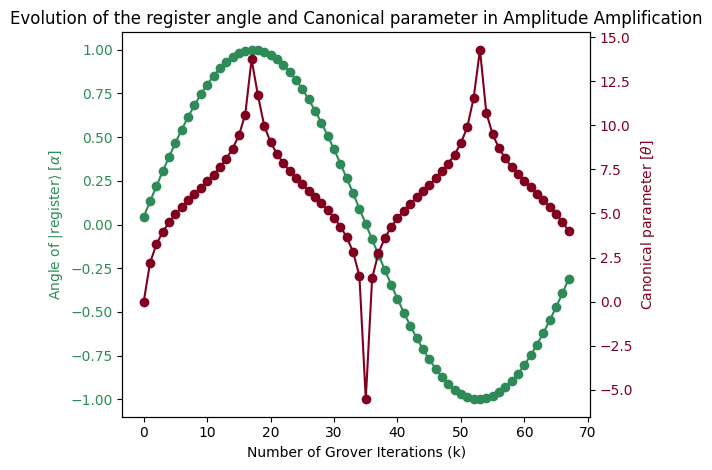
\includegraphics[width=\linewidth]{pics/can_angle.png}
            \label{subfig:can_ANG}
            \end{subfigure}

            \caption{\textbf{Series of Grover rotations on a given logical formula.} The expected shootout in the canonical parameters of the exponential family
            can be seen in both figures. First it is compared to the change in probability, secondly against the angle of the register. The log-odds function, with which we define $\theta_k$, has vertical asymptotes at $P = 0$ and $P = 1$, with the added 
            change in behaviour coming from the non-monotonic, but sinusoidal change of $P_g^k$. This understates those explosive `jumps', as the function reacts 
            extremely to values close to 0 or 1, which shows that with near perfect amplification, when $P_{\mathcal{G}} \rightarrow 1$, we have a local maximum 
            in the canonical parameter.}
            \label{fig:can_changes}

            \end{figure}


            \begin{figure}[H]
            \centering

            \begin{subfigure}{0.65\textwidth}
            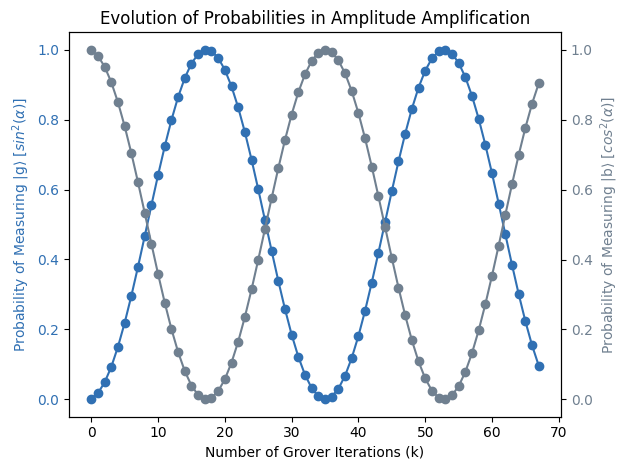
\includegraphics[width=\linewidth]{pics/can_prob_gb.png}
            \label{subfig:can_PROB_gb}
            \end{subfigure}

            \medskip % insert a bit of vertical whitespace
            \begin{subfigure}{0.75\textwidth}
            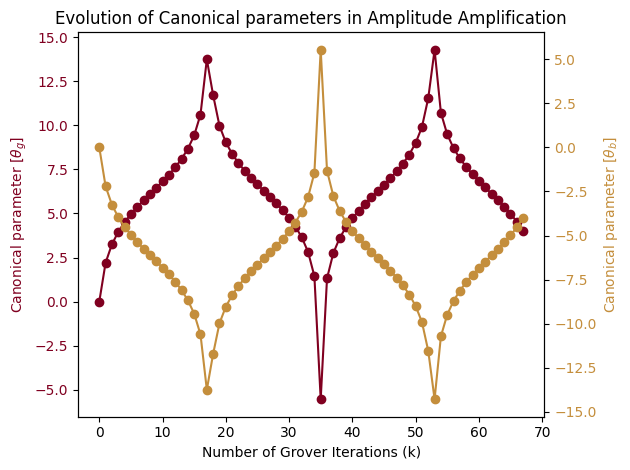
\includegraphics[width=\linewidth]{pics/can_gb.png}
            {\phantomsubcaption\label{subfig:can_ANG_gb}}
            \end{subfigure}

            \caption{\textbf{Probabilities and canonical parameters of the $good$ and $bad$ states.}t is visible, that while the probability of finding a $target$ state, and of not, sums up to one. After each Grover iteration,
            we will have $P_g^i + P_b^i = 1$. The vector of canonical parameters however is unnormalized, as it is just defining relative weights for outcomes.
            The normalization is handled by the log-partition function $A(\theta)$. This not only shows us how the parameters of the underlying exponential family representation are tuned,
            but also serves as a proof, that only the canonical parameter of the formula changed, whilst the sufficient statistics remains the same.}
            \label{fig:can_gb_2}

            \end{figure}

            

    \section{Generalization and Scalability}
    These extended theoretical results are consistent with, and importantly reinforce, the findings from the earlier six-qubit system discussed in Section~\ref{sect:EE_Results}. In the smaller system, 
    the evolution of $P_g^{(k)}$ and $\theta^{(k)}$ closely matched analytic predictions, with the monotonic increase and subsequent overrotation being clearly visible over a few amplification steps. 
    This close correspondence between simulation and theory provided a solid foundation. The extrapolated dynamics for lower target probabilities and additional amplification rotations further validate 
    the robustness and generality of the theoretical framework, even in regimes beyond those directly simulated.

    The repetition of the sinusoidal profile and canonical parameter “explosions” in this setting serves to validate the universality of the amplitude amplification mechanism and its framework via 
    exponential family parameters. It also confirms that the canonical parameterization remains a robust and meaningful descriptor of the distribution throughout the amplification process, regardless 
    of system size. The scalability of these characteristic behaviors confirms that quantum amplitude 
    amplification can serve as an effective primitive within hybrid quantum-classical workflows, feeding back adjusted parameters into classical inference engines.
    The approach thus generalizes to larger logical connectives and higher-dimensional systems. For $n$-qubit systems with more complex formulas, 
    the mapping to exponential families and utilizing slice tensor decomposition remains valid, and the quantum circuit construction follows the same principles.
    Of course real-life scalability is determined by the complexity of the distributions, therefore the circuits, and also the available quantum resources.
    Nevertheless, having these effects observed in a large-scale simulation offers confidence that hardware developments targeting increased qubit counts and connectivity can 
    harness the modeled phenomena to achieve substantive quantum advantage in AI tasks.


\chapter{Benchmarking and Comparative Analysis}
After presenting a small test example for the quantum enhanced sampling procedure, where we have seen the feasibility of the algorithm, we need to turn our attention to 
the speed of the procedure. First it will be checked asymptotically, how it stacks up against classical sampling procedures; then how utilizeable and robust it is on a 
selected current state NISQ platform.

    \section{Classical Sampling Methods}
    \label{sect:Benchmark_classical}
        Sampling is the process of drawing representative instances from a dataset or knowledge base, serving as a fundamental operation in 
        machine learning and artificial intelligence workflows. Classical sampling methods reviewed here include the brute-force enumeration,
        rejection sampling and Markov Chain Monte Carlo (MCMC) methods, each with distinct strengths and limitations~\cite{Ghojogh2020}.
        
        \subsection{Brute-Force Enumeration}
            Brute force sampling, also known as exhaustive enumeration, is the most direct approach to sampling from a probability distribution: 
            it systematically generates and evaluates every possible state in the sample space. For a discrete distribution over $N$ states, this 
            means explicitly listing all $N$ configurations, computing their probabilities, and either selecting samples according to their 
            weights or simply iterating through all possibilities.

            While conceptually simple and guaranteed to be exact, brute force methods are only feasible for very small systems. For problems involving 
            $n$ binary variables, the number of all possible states is $N = 2^n$. Thus the cost grows exponentially with $n$, the time 
            and memory complexity scaling as $\mathcal{O}(2^n)$. This is a classic example of the `curse of dimensionality' or 
            combinatorial explosion.

            Brute force enumeration is sometimes used as a baseline for validating other sampling algorithms or for very small models. 
            However, for most real-world applications, the exponential scaling renders brute force approaches intractable. Even modest 
            increases in $n$ quickly make the approach impractical, motivating the use of more sophisticated methods such as rejection 
            sampling, MCMC, or quantum algorithms.

        \subsection{Rejection Sampling}
            Rejection sampling is a fundamental technique for generating samples from a target distribution $f(x)$ when direct sampling is 
            impractical. The method uses a proposal distribution $g(x)$, from which sampling is easy, and accepts or rejects each candidate 
            based on the ratio $f(x)/(M g(x))$, where $M$ is a constant such that $M \geq \sup_x p(x)/q(x)$ for all $x$. The efficiency of 
            rejection sampling heavily depends on the choice of the proposal distribution; if $g(x)$ poorly approximates $f(x)$, the 
            acceptance rate drops and the method becomes computationally inefficient~\cite{Lee2025}. The coice of said proposal distribution will define the $M$
            value, from which a suitable acceptance rate can be deduced. Despite its simplicity, rejection sampling can be wasteful for 
            high-dimensional or rare-event scenarios, as the expected number of trials to obtain one valid sample scales as $\mathcal{O}(M)$. 
            In rare events, where $P_g$ -- the probability of a \textit{target} state -- is low, matched with a proposal distribution resulting in a 
            high M value $\approx \frac{1}{P_g}$, resulting in a computational complexity of $\mathcal{O}(\frac{1}{P_g})$, which just like with brute-force 
            algorithms, is becoming prohibitive for rare events ($P_g \ll 1$). With an easy-to-sample distribution, or a suitable proposal one, the value for 
            M will be much lower, and the acceptance rate higher. This means in the end a well built rejection sampling can achieve over the previously 
            defined complexity, albeit only by a constant multiplier. 

        \subsection{Markov Chain Monte Carlo (MCMC)}
            MCMC methods, such as the Metropolis-Hastings algorithm and Gibbs sampling, construct a Markov chain whose stationary distribution 
            is the target distribution~\cite{PMC5862921}. By sequentially generating correlated samples, MCMC can explore complex, 
            high-dimensional distributions even when direct sampling or rejection sampling is infeasible. The key advantage of MCMC is its 
            flexibility: it only requires the ability to compute the (unnormalized) density of the target distribution. However, MCMC methods 
            can suffer from slow mixing, especially in multimodal or high-dimensional spaces, and require careful tuning to ensure convergence 
            and independence of samples.
            \\
            MCMC constructs a Markov chain converging to $p(x)$. For Gibbs sampling, with $N$ being the number of possible states:
            \begin{itemize}
                \item Mixing time scales as $\mathcal{O}(e^{N})$ for multimodal distributions
                \item Per-iteration cost: $\mathcal{O}(N)$ for local updates
                \item Suffers from slow mixing in high dimensions due to metastability
            \end{itemize}
            So while classical sampling methods such as brute-force methods, rejection sampling and MCMC are widely used and well-understood, neither method 
            achieves better than linear scaling in $1/P_g$ or exponential in $N$, thus they face significant challenges in the context 
            of high-dimensional, structured, or rare-event distributions.

    \section{Quantum vs. Classical: Asymptotic Speedup}
    \label{sect:Benchmark_asymptotic}
        Quantum amplitude amplification achieves a quadratic improvement, requiring only $\mathcal{O}(1/\sqrt{P_g^0})$ queries. This has been shown by 
        the calculations in section \ref{subsect:QSA_AA_paramupdate} and backed up by a dummy example in section \ref{sect:EE_Results}.
        This follows from Grover's theorem and its generalization to amplitude amplification as defined in sect.~\ref{sect:QSA_AA}:
        \begin{theorem}[Brassard et al. 2000]
        Given an initial state $A|0\rangle$ with good-state probability $P_g^0 = \sin^2\alpha$, after $k = \lfloor \frac{\pi}{4}\sqrt{\frac{1}{P_g^0}} \rfloor$ 
        iterations of $\mathbf{Q} = -\mathcal{A} \mathbf{S}_0 \mathcal{A}^{-1} \mathbf{S}_\chi$, the probability of measuring a good state 
        satisfies:
        \begin{equation}
        P_g^k = \sin^2((2k+1)\alpha) \geq 1 - P_g^0 = P_b^0
        \end{equation}
        \end{theorem}

        \begin{proof}
        The state evolution under $Q$ performs a rotation in a 2D subspace spanned by $|\psi_g\rangle$ and $|\psi_b\rangle$~\ref{subsect:QSA_AA_paramupdate}. 
        After $k$ iterations:
        \begin{equation*}
        Q^k A|0\rangle = \sin((2k+1)\alpha)|\psi_g\rangle + \cos((2k+1)\alpha)|\psi_b\rangle
        \end{equation*}
        Choosing $k = \lfloor \frac{\pi}{4}\sqrt{\frac{1}{P_g^0}} \rfloor$ yields $(2k+1)\alpha \in [\pi/2 - \alpha, \pi/2 + \alpha]$, giving $P_g^k \geq \cos^2\alpha = 1 - P_g^0 = P_b^0$.
        Thus after $k$ iterations we have a probability $P_g^k$ higher than $P_b^0$.
        \end{proof}

        This demonstrates that $\mathcal{O}(1/\sqrt{P_g^0})$ iterations suffice to amplify the success probability near 1, quadratically 
        faster than classical sampling methods.

        \subsection{Full Circuit Depth Analysis}
        Although we see that the amplitude amplification achieves a quadratic improvement over classical algorithms, it is only the
        `search' part of our procedure, and the quantum advantage must account for full circuit depth, not just oracle queries. 
        Thus we need to include the state preparation unitaries as well:
        \begin{itemize}
            \item $D_A$: Depth of state preparation circuit
            \item $D_O$: Depth of oracle implementation
            \item $D_D$: Depth of diffusion operator
        \end{itemize}
        The total depth for $k$ iterations is:
        \begin{equation}
        D_{\text{total}} = D_A + k(D_O + D_D)
        \end{equation}

        Which in my implementation sums up to:
        \begin{itemize}
            \item Uniform preparation: $D_A = \mathcal{O}(n)$ $\rightarrow$ Hadamard gates on all qubits are $\mathcal{O}(1)$ with utilizing paralellism
            plus NOT/Toffoli gates for logical formula mapping are $\mathcal{O}(cn)$
            \item Logical oracle: $D_O = \mathcal{O}(1)$ $\rightarrow$ as only a single $\hat{Z}$ gate is applied on the \textit{indicator qubit} 
            (as it represents the whole logical formula).
            \item Diffusion: $D_D = \mathcal{O}(2n)$ (essentially overlapping with the state preparation unitary)
        \end{itemize}

        Thus the total depth of the circuit comes down to:
        \begin{align*}
            D_{\text{total}} &= \mathcal{O}(n + k(2n+1)) \\
            \intertext{which equals for $k \approx 1/\sqrt{P_g^0} = \sqrt{2^n} = 2^{n/2}$}
            D_{\text{total}} &= \mathcal{O}(n + 2^{n/2}(n+1)) \\
            D_{\text{total}} &\approx \mathcal{O}(n \cdot 2^{n/2})
        \end{align*} 
        The quantum method gives a quadratic (square-root) speedup asymptotically when put up against the classical sampling methods listed in sect.~\ref{sect:Benchmark_classical}.


\section{Resource Estimation and Practical Feasibility}
The choice of quantum hardware platform is a critical factor in translating theoretical quantum speedup into practical, 
real-world performance. Different technologies offer distinct trade-offs in terms of gate speed, fidelity, connectivity,
and scalability. These properties directly affect the feasibility and efficiency of implementing quantum algorithms, such as 
the proposed sampling procedure.
    \subsection{Platform proposal}
    The selection of a quantum hardware platform should be guided by the specific requirements of the task at hand. For this 
    thesis, the focus is on sampling from complex logical connectives and exponential family distributions with utilizing 
    amplitude amplification, i.e. repeated Grover's algorithm. When evaluating platforms for such algorithms that
    require deep circuits and many multi-qubit entangling gates, key considerations include:

    \begin{itemize}
        \item \textbf{Gate Fidelity and Error Rates:} High-fidelity gates are essential to maintain coherence and ensure the 
        reliability of sampling results, especially as circuit depth increases.
        \item \textbf{Coherence Times:} Longer coherence times allow for more complex algorithms to run without significant 
        decoherence, which is crucial for amplitude amplification and other iterative procedures.
        \item \textbf{Qubit Connectivity:} All-to-all connectivity enables direct entanglement between any pair of qubits, 
        reducing the need for SWAP gates and simplifying circuit compilation for highly non-local operations.
        \item \textbf{Native Gate Set:} The availability of native multi-qubit gates or efficient decomposition of logical 
        operations can greatly affect the overall circuit depth and execution time.
        \item \textbf{Scalability:} The ability to scale up to larger numbers of qubits without a significant drop in 
        performance is important for tackling high-dimensional sampling problems.
    \end{itemize}

    \vspace{1em}
    \noindent
    \textbf{Platform Selection Rationale}

    While superconducting qubit platforms offer fast gate times and are widely accessible~\cite{Huang_2020}, their limited qubit connectivity (nearest neighbour) 
    and shorter coherence times can become bottlenecks for deep or highly connected circuits. In contrast, trapped ion quantum computers~\cite{bernardini2023quantumcomputingtrappedions} 
    provide several compelling advantages for this class of problems:

    \begin{itemize}
        \item \textbf{All-to-All Connectivity:} Eliminates the need for SWAP gates, allowing direct implementation of multi-qubit 
        logical connectives and reducing compilation overhead.
        \item \textbf{Superior Gate and Measurement Fidelity:} Minimizes cumulative error, making it feasible to execute longer 
        circuits with high accuracy.
        \item \textbf{Native support for multi-qubit gates:} Some platforms implement multi-qubit entangling gates directly, 
        further reducing circuit depth for logical oracles and diffusion operators.
        \item \textbf{Exceptionally Long Coherence Times:} Supports deep amplitude amplification sequences and complex sampling 
        routines without significant loss of quantum information.
        \item \textbf{Scalability:} Recent advances have demonstrated the ability to operate with dozens of qubits, with roadmaps 
        to even larger systems.
    \end{itemize}

    So, although superconducting qubits have been the workhorse of many quantum computing experiments, trapped ion platforms are 
    particularly well-suited for quantum sampling tasks that involve high circuit depth and complex logical structure. 
    For these reasons, it is the platform, which poses as the most well-suited choice for the quantum samplig algorithm. Trapped ion 
    platforms are quite accessible as well, with many instances being provided by individual companies and research groups. The following 
    table details the relevant hardware specifications and performance characteristics of trapped ion quantum computers, providing a concrete foundation 
    for resource estimation and benchmarking of the proposed quantum sampling algorithms.

    It is important to emphasize that generic quantum circuits must be transpiled to run efficiently on trapped ion platforms. Transpilation converts a circuit 
    into an equivalent sequence of gates native to the hardware, such as single-qubit GPI/GPI2 gates and multi-qubit Mølmer-Sørensen (MS) gates. In my case, 
    this process has significantly increased the number of gates compared to the original logical gate count - a \textit{constant} factor that was not fully accounted for in the 
    initial resource and turnover time calculations. Nevertheless, the total gate count after transpilation remains comparatively low, primarily due to the 
    intrinsic all-to-all connectivity feature of trapped ion systems, which eliminates the need for costly SWAP gates required on other architectures with 
    limited qubit connectivity. Thus, despite the gate count increase from transpilation, trapped ion platforms maintain a substantial advantage for 
    implementing highly entangled circuits such as those used in amplitude amplification, where alternate platforms would suffer from a heavy overhead due 
    to numerous SWAP operations.

\subsection{Circuit Compilation and Scaling}

For a general $n$-variable logical formula (with $N = 2^n$ states and one \textit{target} state, $p_g = 1/N = \frac{1}{2^n}$) the depth is:
\begin{equation*}
    D_{\text{total}} \approx \mathcal{O}(n \cdot 2^{n/2})
\end{equation*}
following our calculations in sect.~\ref{sect:Benchmark_asymptotic}.

\noindent
\textbf{Transpilation Considerations:}  
Although some logical gates (e.g., Toffoli, multi-controlled $\hat{Z}$) are not native to trapped ion hardware, all-to-all connectivity and 
high-fidelity two-qubit gates enable efficient transpilation. The absence of SWAPs and the possibility of direct multi-qubit entangling gates 
(e.g., Mølmer–Sørensen) mean that even transpiled circuits remain shallow compared to superconducting platforms for the same logical depth,
even with the previously mentioned gates being native on such platofmrs.

\subsection{Quantum vs. Classical Runtime Scaling}

For a target probability $P_g^0 = 1/2^n$:

\begin{itemize}
    \item \textbf{Classical sampling (brute force or rejection):}
        \[
        T_{\text{classical}} = \frac{1}{P_g^0} \cdot t_c = 2^n \cdot t_c
        \]
        where $t_c$ is the classical step time (e.g., $1$ ns). Rejection sampling only differs
        from this with a constant multipier.
    \item \textbf{Quantum amplitude amplification:}
        \[
        T_{\text{quantum}} = \frac{1}{\sqrt{P_g^0}} \cdot D_{\text{iter}} \cdot t_g = 2^{n/2} \cdot n \cdot t_g
        \]
        where $t_g$ is the quantum gate time.
\end{itemize}

\subsection{Turnover Point Analysis}

Quantum advantage is achieved when $T_{\text{quantum}} < T_{\text{classical}}$, or:
\[
2^{n/2} \cdot (1 + 2n) \cdot t_g < 2^n \cdot t_c
\]
Single qubit gate times are tens of microseconds to about 50 microseconds on average, while two-qubit gates take 50-500 microseconds typically.
Thus a crossover point can be approximated on average as:
\[
10^5 \cdot (1 + 2n) < 2^{n/2}
\]

\textbf{Numerical solution:}
\begin{itemize}
    \item For $n=30$: $10^5 \times 61 = 6.1 \times 10^6 < 2^{15} = 32,768$ (not yet quantum-advantaged)
    \item For $n=40$: $10^5 \times 81 = 8.1 \times 10^6 < 2^{20} = 1,048,576$ (not yet quantum-advantaged)
    \item For $n=50$: $10^5 \times 101 = 1.01 \times 10^7 < 2^{25} = 33,554,432$ (close to quantum advatage)
    \item For $n=60$: $10^5 \times 121 = 1.21 \times 10^7 < 2^{30} = 1,073,741,824$ (quantum is much faster)
\end{itemize}

\noindent
\textbf{Conclusion:} The quantum-classical turnover for rare-event sampling occurs at \linebreak $n \approx 50$ qubits on current 
trapped ion hardware.  

\subsection{Performance on trapped ion hardware}

Trapped ion quantum computing exhibits distinctive performance characteristics across several key metrics. Coherence times for trapped ion qubits can reach up to about 
60 seconds in the best cases, often spanning several seconds to tens of seconds on average, with worst-case coherence times still substantially longer than those of many 
other qubit platforms. Single-qubit gate times typically range from around 1 microsecond in optimized setups to tens of microseconds on average, with worst-case times 
extending into hundreds of microseconds. Two-qubit gate times are generally longer, spanning from approximately 1 microsecond for advanced pulse-controlled gates up to 
hundreds of microseconds or milliseconds depending on system specifics and operations involved.

Gate fidelities on trapped ion devices are among the highest in quantum computing. Single-qubit gates can achieve fidelities up to 99.9999\%, with averages commonly 
between 99.5\% and 99.99\%, while worst-case fidelities remain above 99\%. Two-qubit gates exhibit best-case fidelities exceeding 99.9\%, averages in the 97.5\% to 99\% 
range, and worst cases around 95\%, with ongoing research pushing these numbers higher.

These performance metrics illustrate the practical advantages and challenges of trapped ion quantum computing, including long coherence times and high-fidelity gates 
enabling low-error, relatively fast quantum sampling compared to classical methods. However, gate times - especially for two-qubit operations - remain slower than some 
other qubit technologies.
\\

\textbf{Performance and feasibility of the test example}
            
The complete algorithm (test example in chapter~\ref{chapter:4}, state preparation and 6 rounds of amplification) includes around 8500 single-qubit gates (\texttt{gpi} and \texttt{gpi2}) and 1200 two-qubit \texttt{ms} gates. Assuming typical trapped ion gate durations of 
approximately 20 microseconds per single-qubit gate and 200 microseconds per two-qubit gate, the total execution time could be held under a few seconds,
a number that comfortably fits within the coherence window of average trapped ion platforms. 

In terms of fidelity, single-qubit gates on trapped ion hardware typically achieve fidelities between 99.5\% and 99.99\%, whereas two-qubit gates range from about 97.5\% to 99.9\%. 
Although the large number of gates compounds errors, the overall fidelity is expected to remain within practical limits for near-term quantum experiments.

In conclusion, the algorithm's duration is compatible with the coherence times of trapped ion qubits, and its fidelity lies within acceptable bounds given current hardware capabilities.

\pagebreak
\subsection{Weak points and Possile improvements}

To improve practical quantum advantage in sampling on trapped ion hardware, the following strategies could be considered:
\begin{itemize}
    \item \textbf{Two-qubit fidelities:} Single-qubit gates have achieved great fidelity, focusing research and engineering efforts on increasing two-qubit gate fidelity is critical. Their precision is not lacking compared
    to other quantum hardware, but with our procedure, where numerous two-qubit gates are utilized, their inaccuracy can lead to fidelity issues. Advancements could involve better pulse shaping, 
    error correction codes designed for two-qubit gates, and refined calibration methods tailored for the ion trap environment.
    \item \textbf{Two-qubit gate times:} Concerning the gate times two-qubit gates can be considered slow compared to other platforms, which can cause issues in deep circuits. Advances in pulse 
    engineering, mode shaping could shorten gate times, nevertheless the high coherence times can make up for it in the long run.
    \item \textbf{Coherence times:} Substantially longer than those of many other qubit platforms, nevertheless by leveraging advanced manufacturing, cryogenic cooling, and improved vacuum 
    or shielding technology can further lengthen the trapped ion coherence times.
\end{itemize}

\noindent
\textbf{Summary:} Trapped ion quantum hardware provides a compelling platform for quantum-enhanced sampling, particularly for deep circuits and rare-event problems. The combination of all-to-all 
connectivity, long coherence times, and ultra-high gate fidelities offsets the slower gate speeds compared to superconducting qubits. As a result, quantum advantage for sampling is projected to emerge at 
$n \geq 50$ qubits for unstructured search, and significantly earlier for structured or highly parallelizable logical connectives. These features make trapped ion systems especially attractive for scalable 
quantum machine learning and probabilistic inference in the near future.

\chapter{Discussion}
\label{chap:Discussion}

    \section{Overview: Contributions within Artificial Intelligence}
    The findings of this thesis open up a possible solution for the growing challenges in modern machine learning and artificial intelligence. As 
    the algorithmic capability increases, so does the computational depth of the tools required for working with high-dimensional, complex data. 
    Sampling problems cut to the core of numerous applications, from Bayesian inference and generative modeling to combinatorial optimization and 
    decision making under uncertainty. 
    
    This thesis brings two major contributions to said matter. The first is the theoretical framework developed, combining exponential 
    families and tensor networks, providing a pathway for mapping structured knowledge bases directly onto quantum states and circuits. This 
    mapping to a quantum circuit is not only unified and applicable to knowledge bases used in ML and AI workflows, but also enables quantum 
    procedures on the data.
    This leads to the other major result of this thesis, a promising new paradigm: quantum-enhanced sampling with amplitude amplification.

    The contributions set up experimentation, comparison, and benchmarking of quantum routines not only against classical baselines, but as 
    foundational components for future hybrid workflows in probabilistic AI.
    
    \section{Scientific Results}
        The first contribution's result is the unified framework linking classical and quantum domains. It makes use of exponential family distributions and tensor networks as an essential bridge 
        between the domains. Exponential families bring together a wide range of probabilistic models/distributions, such as Bernoulli, Binomial, Gaussian; as well as propositional logical 
        formulas and probabilistic graphical models. These admit to both canonical ($\theta$-parametrized) and mean-parameter ($\mu$-parametrized) dual descriptions. 

        Slice tensor decomposition serves two roles: enabling classical scalability for inference and learning by compressing or “slicing” high-dimensional distributions into manageable factors, 
        i.e. slices; and providing a baseline for quantum circuit implementation where local structure is mapped to quantum gates or registers. For example, in models with conditional 
        independence, the decomposition reveals which variables/parameters admit efficient, parallel encoding, thus minimizing the need for multi-qubit - and thus error-prone - entangling gates.

        A other key result of this thesis is the possibility of a quantum sampling procedure, and the careful quantification of a speedup compared to classical algorithms. While prior research has highlighted the quadratic 
        advantage for amplitude amplification, this work pushes further, showing an application for the procedure and highlighting how and where quantum algorithms can operate more efficiently. The 
        quadratic reduction in sampling cost (from $\mathcal{O}(1/P_g^0)$ to $\mathcal{O}(1/\sqrt{P_g^0})$ for events of probability $P_g^0$) is confirmed for structured examples 
        and extended to general exponential family representations.

        \subsection*{Empirical Validation and Scalability}
        Through implementation of quantum sampling routines on up to about 28 qubits using classical simulators, the thesis provides valuable 
        empirical validation  - as the test problem in Chapter \ref{chapter:4}. 
        Notably, by integrating classical circuit-depth analysis with practical quantum implementation (including full gate counts and state preparation costs), the thesis 
        finds the crossover point between quantum and classical speeds and accuaricies. This depends on problem size and problem structure (i.e. dimension and structure of the knowledge base), as well as hardware overheads.
        The benchmarking results indicate that quadratic speedups are realized in practice for target-finding problems, and that the expected “turnover point” where quantum methods become faster than 
        classical procedures appears within reach as quantum hardware matures. The observed scaling laws for circuit depth, probability amplification, and resource consumption match theoretical predictions.
 
        For low-dimensional models, possibly with independent variables and high $target$ probabilities (just like the dummy example of a joint Bernoulli distribution throughout the thesis), 
        quantum methods are efficient but not necessarily advantageous; the speedup emerges decisively for 
        high-dimensional, and rare-event sampling tasks where brute-force, classical rejection or Markov Chain Monte Carlo (MCMC) approaches are exponential in scaling or poorly mixing.

        Additionally, the analysis of hardware requirements, like gate fidelities, coherence times, qubit overhead, error rates; offers actionable insights for experimentalists aiming to demonstrate 
        quantum advantage in real-world AI-relevant sampling contexts.

    \section{Implications for quantum enhanced AI}
        \subsection{Unifying Symbolic and Probabilistic Reasoning}
        One of the more subtle implications of this research comes from the fact that logical formulas (e.g., propositional logic, rules, constraints) and probabilistic models (e.g., graphical models, 
        exponential families) can be handled by a unified tensor network formalism. In classical contexts, this enables the growing field of neuro-symbolic AI; melding logical reasoning with probabilistic inference. 
        Quantum computation adds a further layer, allowing these unified models to be encoded, evolved, and measured as quantum states.

        This unification is not merely aesthetic. By developing a mathematical framework that represents both logical formulas and probabilistic models as tensor networks, the thesis makes this integration explicit. 
        This common representation enables leveraging tensor decomposition techniques to break down complex knowledge bases - comprised of logical connectives, rules, and probabilistic relationships - into factors that 
        can be handled uniformly. The work bridges a gap between classical AI representations and scalable quantum algorithms it allows for new workflows in knowledge discovery, automated theorem proving, and scientific 
        reasoning where uncertainties are both explicitly modeled and efficiently sampled in ways robust to high-dimensional or combinatorial structure.

        \subsection{Hardware Roadmaps and Near-Term Opportunities}
        The resource analysis in this thesis suggests that, while current superconducting and trapped ion platforms are still challenged by noise, scalability, and depth, the hardware gap is shrinking. 
        All-to-all connectivity in trapped ion systems, advances in error mitigation, and growing industry roadmaps mean that quadratic quantum speedups for sampling may be demonstrated in prototype tasks 
        within a few years, maybe even for larger systems, with greater depth/number of qubits. Industry leading trapped ion platforms have roadmaps containing 10,000 physical qubits on a single 
        chip, and $99.9\%+$ two-qubit gate fidelity on development and commercial systems. And this maturing in hardware is due to arrive within a few years \cite{ionq_roadmap}.

        This is especially relevant for domains such as finance, logistics, and scientific simulations, where sampling rare events from highly-structured models is core to risk estimation, optimization, 
        and planning. The methods and mappings detailed in the thesis can be directly transfered to such settings.

        \subsection{The Path to Hybrid Quantum-Classical AI}

        Another key opportunity is the integration of quantum sampling modules into classical ML/AI workflows. Several computational models and paradigms could be imagined:
        \begin{itemize}
            \item Pre-conditioning classical probabilistic models with quantum-sampled data. As the procedure presented here not only samples the knowledge base but also modifies distribution parameters 
            just like classical iterative parameter update schemes. Thus a bias will be introduced towards $target$ states, which pre-conditions the classical model to easier further sampling.
            \item Hybrid inference pipelines where challenging components (such as hard constraints or rare events) are delegated to quantum processors, while routine inference remains classical.
            Or even better, adaptive algorithms, where quantum hardware co-processors are triggered “on demand” when classical samplers fail due to exponential bottlenecks or poor mixing.
            This depends wether we are sampling from a knowledge base manageable by classical methods, or if quantum takeover is needed. For multivariate distributions certain parts could be 
            handled by classical methods, whilst the harder, classically unfeasible elements should be handed over to an on-demand quantum processing unit.
        \end{itemize}
        The TNREASON framework and associated software developed in this research are important steps toward such hybrid modalities. As knowledge bases are represented classically, with logical formulas,
        or probabilistic graphical models, built in tensor contraction features, and easy to apply classical sampling processes are applicable. Nevertheless with the new paradigm of quanum enhanced sampling involved,
        we can switch between the two easily, as the same knowledge base representation is utilized, thus it is only a question of preference (and of course computational need).

    \section{Limitations and Open Challenges}
    Although the proposed algorithm is promising, and with current state hardware maturing real-life tests and utilization is on the boeard, critical evaluation reveals several hurdles from both the theoretical
    and the practical sides.

        \subsection*{Theoretical and Algorithmic Limits}
        \begin{itemize}
            \item \textbf{Limited to Quadratic Speedup:} Amplitude amplification and Grover-like algorithms do not (in the black-box regime) break the quadratic speedup barrier. For many ML tasks, full exponential 
            speedup remains out of reach, though there is scope for greater than quadratic advantage in structured or oracle-learnable settings.
            \item \textbf{Fast classical algorithms:} Not only quantum algorithms have the opportunity to keep on getting faster. Some modern classical sampling algorithms, such as advanced MCMC variants or variational 
            approaches, may close much of the gap to quantum acceleration - especially for distributions with tractable structure or learnable proposal mechanisms. Thus breaking the quadratic speedup barrier is not only about 
            researching various quantum procedures, but also about making quantum improve faster than the classical algorithms are improving.
            \item \textbf{Real-World Integration:} Even when quantum sampling is theoretically advantageous, real datasets often require extensive data encoding, classical postprocessing, and integrated workflow 
            design to ensure that quantum routines genuinely drive end-to-end capability improvement. This problem could be adressed by a more robust decomposition technique, so that classical datasets can fit easier into quantum workflows.
        \end{itemize}

        \subsection*{Practical Hardware Bottlenecks}
        \begin{itemize}
            \item \textbf{Noise and Decoherence:} Even minor gate errors accumulate rapidly in deep circuits. For amplitude amplification, Grover’s iteration is applied $k$ times. Therefore the Diffuison operator \textbf{D} - which is assembled from
            the state preparation and its inverse - is applied $k$ times, meaning the state preparation unitary are applied $2k$ times.      
            With the vast number of gates, cumulative errors can overwhelm the quadratic speedup, leading to practical constraints on feasible problem sizes in current-state NISQ (Noisy Intermediate-Scale Quantum) devices. 
            Improvements in gate fidelities, or/and in error-correction are needed in the long run, so the number of gates will not be an issue.
            \item \textbf{Oracle complexity:} Of course the amplitude amplification algorithm requires $k$ applications of the Oracle \textbf{O} as well. For non-trivial logical formulas or multi-level constraints a `simple' 
            oracle might not suffice as it did here. An efficient phase oracle circuit (that marks the “good” states) is neeeded, although that may require complex ancilla management, multi-controlled Toffoli gates, or large 
            numbers of ancillary qubits. Each adds both gate count and error vulnerability. It could be overcome by automated or semi-automated construction of complex quantum oracles that recognize (or mark) all solutions.
            For example, with the utilization of an ancillary qubit for the indicator function - just like we have done with the \textit{indicator qubit}, the depth can be greatly reduced.
            \item \textbf{Scalability to Arbitrary Graphs/Models:} Not all classical models decompose compactly or admit efficient tensor network representations. Dense graphical models or highly entangled 
            logical connectives may remain intractable even for quantum routines unless further innovations in model structure, parameterization, or circuit compilation are developed.
        \end{itemize}

    \section*{6.5 Future Research Directions}
    Inspired by results and challenges above, exciting paths for continued research include:
    \begin{itemize}
        \item \textbf{Development of more expressive and resource-efficient tensor network decompositions.} The slice tensor decomposition utilized in the thesis proved to be useable with both the dummy example and the test knowledge base. 
        As an advancement, the mapping of complex distributions to quantum states and circuits could be more straightforward and robust. This can achieved with numerous tests, where more complex, higher dimensional
        knowledge bases would undergo the mapping procedure, through slice-decomposing their exponential family representation. Then, a picture can be obtained about the hardships and challanges about mapping
        highly dependent and intricate structures. This question however is not only about the decomposition itself but the mapping of these structures too, and the representation of structure as quantum operations (gates).
        \item \textbf{Mapped quantum states with a generalized gate set.} To follow up from before, a robust decomposing/mapping algorithm could use a pre-defined set of gates ($\mathbf{\hat{X}}$, $\mathbf{C\hat{X}}$, $\mathbf{MC\hat{X}}$) to encode probabilities/amplitudes and dependencies within the knowledge base.
        The selected gate-set depends on both the structure of the knowledge base, but also the selected quantum platform to be utilizied. With a well defined and carefully selected set, quantum parallelism could be exploited, the gates with the best parameters - such as fidelity, gate-time - could 
        be selected. This way a more precise decomposing and sampling algorithm could be used, that might be able to reach quadratic speedup on smaller systems even. As with amplitude amplification quadratic speedup remains the ceiling of our possibilities, but the turnover point could come sooner, with even less qubits.
        Another way would be using purely Rotation gates, where we can have precise algorithms on the trapped-ion platforms.
        \item \textbf{Experimental validation on near-term quantum hardware.} A future goal is to generate full-stack benchmarks for both classical and quantum sampling (as hardware matures). Therefore, a clearer picture would be obtained about the speed difference between classical and quantum.
        With full-stack benchmarks the precision, the robustness and the scalability of the algorithm can be modelled on current state quantum platforms. It would give a clear picture about the current state of platforms, including runtimes and fidelity, as well as the feasibility of the procedure as of now.
        Also future platform   
        \item \textbf{Investigations into non-standard quantum sampling primitives.} These may surpass quadratic speedup in restricted or adaptive settings (e.g., quantum walks, adiabatic quantum computation, or quantum Boltzmann machines).
        Higher dimensional sampling issues could be restricted to ancillas, where the amplification would only be made on such final connective qubits, representing the whole distibution.
        \item \textbf{Applications in other domains.} Beyond the example and toy models, direct deployment can be informative in financial data analysis, logistics, computational biology, or AI-driven scientific discovery. It is in order specifically in areas where high-dimensional structured sampling is a limiting factor.
    \end{itemize}

    \section*{6.6 Conclusions and Outlook}
    This thesis advances the field by unifying classical representations and quantum implementation of probabilistic and logical models, providing a systematic method for quantum circuit mapping via tensor networks, and empirically verifying quadratic speedups for critical sampling tasks. 
    By quantifying resource demands, identifying the classical to quantum turnover point, and analyzing the role of hardware design, this work builds a bridge between promising quantum theory and future AI applications.

    Looking ahead, the role of quantum sampling in AI will likely expand as hardware improves, hybrid paradigms mature, and as real-world bottlenecks in classical probabilistic inference demand fundamentally new computational processes. The duality between logic, probability, tensors, and 
    qubits explored here lays groundwork for a new generation of robust, expressive, and scalable machine learning architectures - where quantum computation is not only an add-on but a core enabler for future artificial intelligence.



\appendix
    %\chapter{Supplementary Material}
    \chapter{Code Listings}
    \label{Appendix_pseudocodes}
    
    \begin{algorithm}[H]
    \caption{Logical Expression to Quantum Circuit Mapping}
    \label{alg:LogicalToQuantum}
    \begin{algorithmic}[1]
    \Function{LogicalToQuantum}{$expression$}
        \Comment{Automatically maps logical expressions to quantum circuits with dynamic qubit allocation}
        \State $variables \gets$ \texttt{extract\_variables}($expression$)
        \State $num\_ancilla \gets$ \texttt{count\_connectives}($expression$)
        
        \State $var\_list \gets$ sorted list of $variables$
        \State $qubits\_map \gets \{$ assign index for each $var \in var\_list \}$
        \State $ancilla\_start \gets$ length of $qubits\_map$
        \State $ancilla\_map \gets \{ \text{'anc'}_{i+1} : ancilla\_start + i \mid i = 0, \ldots, num\_ancilla-1 \}$
        \State Update $qubits\_map$ with $ancilla\_map$
        
        \State $circuit \gets$ new \texttt{QuantumCircuit}()
        \For{each $name$ in sorted $variables$}
            \State $qreg \gets$ \texttt{QuantumRegister}(1, name=$name$)
            \State Add $qreg$ to $circuit$
        \EndFor
        
        \State $anc\_reg \gets$ \texttt{QuantumRegister}($num\_ancilla$, name=\text{"anc"})
        \State Add $anc\_reg$ to $circuit$
        
        \State $basis\_qubits \gets$ indices of logical $variables$
        \For{each $q$ in $basis\_qubits$}
            \State Apply Hadamard gate to qubit $q$ in $circuit$
        \EndFor
        
        \State $ancilla\_counter \gets [0]$ \Comment{mutable counter}
        \State $final\_result \gets$ \texttt{resolve\_expression}($expression$, $circuit$, $qubits\_map$, $ancilla\_start$, $ancilla\_counter$)
        
        \State \Return $circuit, qubits\_map$
    \EndFunction
    \end{algorithmic}
    \end{algorithm}

    This algorithm takes a logical expression as input and automatically maps it onto a quantum circuit. 
    
    It first extracts all the logical variables 
    and counts the number of logical connectives to determine how many ancillary qubits will be needed. It then assigns indices to the variables and 
    ancilla qubits, creating a map for qubit allocation. The quantum circuit is built dynamically with one quantum register per variable and an 
    additional register for the ancilla qubits. The dynamic allocation not only makes it robust, but when going through the circuit we can easily check 
    if the qubits and gates have been applied precisely, by following the names of variables and allocated qubits. 
    
    For the state preparation Hadamard gates are applied to all basis qubits to create superposition states. Finally, the expression is recursively 
    resolved into quantum gates through the $resolve \_ expression$ function~\ref{alg:ResolveExpression}, producing a quantum circuit that represents the whole logical function. 

    \begin{algorithm}[H]
    \caption{Resolve Logical Expression to Quantum Gates}
    \label{alg:ResolveExpression}
    \begin{algorithmic}[2]
    \Function{ResolveExpression}{$expr, circuit, qubits\_map, ancilla\_start, ancilla\_counter$}
        \Comment{Recursively resolve nested logical expressions into quantum gates}
        \If{$expr$ is a variable (string)}
            \State \Return $qubits\_map[expr]$
        \EndIf

        \If{$expr$ is a list with length $> 1$}
            \State $gate \gets expr[0]$ \Comment{Logical connective}
            \State $args \gets expr[1:]$
            
            \State $resolved\_args \gets \emptyset$
            
            \State $target \gets ancilla\_start + ancilla\_counter[0]$
            \State Increment $ancilla\_counter[0]$ by 1
            
            \If{$gate = \text{"not"}$ and length of $resolved\_args = 1$}
                \State Apply $\mathbf{not}$ gateset on $resolved\_args[0]$ to $target$
            
            \ElsIf{$gate = \text{"and"}$ and length of $resolved\_args = 2$}
                \State Apply $\mathbf{and}$ gateset on $resolved\_args[0]$ to $target$
            
            \ElsIf{$gate = \text{"or"}$ and length of $resolved\_args = 2$}
                \State Apply $\mathbf{or}$ gateset from $resolved\_args[0]$ to $target$
            
            \ElsIf{$gate = \text{"xor"}$ and length of $resolved\_args = 2$}
                \State Apply $\mathbf{xor}$ gateset from $resolved\_args[0]$ to $target$
            
            \ElsIf{$gate = \text{"implication"}$ and length of $resolved\_args = 2$}
                \State Apply $\mathbf{implication}$ gateset on $resolved\_args[0]$
            
            \ElsIf{$gate = \text{"bijection"}$ and length of $resolved\_args = 2$}
                \State Apply $\mathbf{bijection}$ gateset from $resolved\_args[0]$ to $target$
            
            \Else
                \State \textbf{Raise an error:} Unknown or improperly formatted gate
            \EndIf
            
            \State \Return $target$
        \EndIf
    \EndFunction
    \end{algorithmic}
    \end{algorithm}

    This algorithm recursively translates a nested logical expression into corresponding quantum gates within a quantum circuit. It handles base 
    cases where the expression is a simple variable by returning its mapped qubit index. For compound expressions, connectives represented as lists, it identifies 
    the logical connective (such as `not', `and', `or' etc.) and recursively resolves each argument. Ancillary qubits are dynamically allocated to 
    store intermediate results, ensuring no qubit position conflicts. Based on the logical connective, the algorithm applies the appropriate quantum 
    gate operations to the resolved argument qubits and ancilla, effectively constructing the quantum circuit equivalent of the logical formula. If 
    an unknown or malformed gate is encountered, the algorithm raises an error, maintaining robustness. This process enables systematic conversion 
    from classical logic expressions to quantum gate implementations.

    \begin{algorithm}[H]
    \caption{Oracle Construction}
    \label{alg:oracle1}
    \begin{algorithmic}[3]
    \Function{Oracle1}{$input\_circ$}
        \State $n \gets input\_circ.\text{num\_qubits}$
        \State $b1 \gets$ Quantum circuit on $n$ qubits
        \State Apply $Z$ gate to $b1$ on qubit $(n-1)$
        \State \Return $b1$
    \EndFunction
    \end{algorithmic}
    \end{algorithm}

    For our case a simple Z gate on the final ancilla qubit - the \textit{indicator qubit} - is enough to `mark' the \textit{target} state. This construction for the circuit, where the indicator function
    is represented as the \textit{indicator qubit} helps us to perform less complex oracles, as the \textit{target} states are those that give 1 for the indicator function - i.e. the \textit{indicator qubit} is in state $\ket{1}$. 

    \begin{algorithm}[H]
    \caption{Quantum Diffusion Operator Construction}
    \label{alg:diffusion}
    \begin{algorithmic}[4]
    \Function{Diffusion}{$input\_circ$}
        \State $n \gets input\_circ.\text{num\_qubits}$
        \State $b1 \gets$ Quantum circuit on $n$ qubits
        \State $b2 \gets b1$ composed with $input\_circ^{-1}$
        \For{$qubit$ in $0, 1, \ldots, n-1$}
            \State Apply $X$ to $b2$ on $qubit$
        \EndFor
        \State Apply $H$ to $b2$ on qubit $(n-1)$
        \State Apply $MCX$ (multi-controlled X) to $b2$ controlled by qubits $0$ to $n-2$, targeting qubit $n-1$
        \State Apply $H$ to $b2$ on qubit $(n-1)$
        \For{$qubit$ in $0, 1, \ldots, n-1$}
            \State Apply $X$ to $b2$ on $qubit$
        \EndFor
        \State $diffusion \gets b2$ composed with $input\_circ$
        \State \Return $diffusion$
    \EndFunction
    \end{algorithmic}
    \end{algorithm}

    The diffusion operator is constructed from the state preparation unitary $\mathcal{A}$. As it is constructed from a sequence of unitary gates, it itself is
    unitary and thus reversible. The diffusion operator therefore follows the paragrph and the equation~\ref{eq:diffusion}, being assembled from the inverse of 
    the state preparation unitary, a rotation around the mean amplitude of all possible n-qubit states, then the preparation unitary again. Thus this implementation 
    is robust for any state preparation unitary and number of qubits.

    \begin{algorithm}[H]
    \caption{Grover Iterations with Oracle and Amplifier}
    \label{alg:applysunscreen}
    \begin{algorithmic}[5]
    \Function{ApplyAmplification}{$circuit$, $oracle$, $amplifier$}
        \State$rounds \gets k$
        \For{$i = 1$ to $rounds$}
            \State $circuit \gets circuit$ composed with $oracle$ composed with $amplifier$
        \EndFor
        \State \Return $circuit$
    \EndFunction
    \end{algorithmic}
    \end{algorithm}

    Finally the Oracle \textbf{O} and Diffusion \textbf{D} operators are applied in sequence for $k$ number of times. 
    It is according to the calculations in eq.~\ref{eq:needed_k}, as per $k = \lfloor \frac{\pi}{4} \sqrt{\frac{1}{P_g^0}} \rfloor$.



\backmatter
\printbibliography

\end{document}